\chapter{Metodologia}\label{cap:metodologia}

Este capítulo descreve como a comparação entre as arquiteturas de aquisição é
conduzida experimentalmente. Apresenta-se primeiro a visão geral do método,
junto com a bancada experimental e o hardware utilizado
(Seção~\ref{sec:bancada}), seguidos da implementação de cada firmware
(Seções~\ref{sec:firmware-a} e~\ref{sec:firmware-b}), das métricas e
procedimentos adotados em cada experimento (Seção~\ref{sec:metricas}) e da
análise estatística (Seção~\ref{sec:analise-estatistica}).

\section{Visão geral do método}

Este trabalho conduz uma comparação experimental controlada entre duas
arquiteturas de firmware de aquisição executando sobre o mesmo hardware, o
mesmo protocolo de \emph{host} e as mesmas condições de teste. O foco central é a
análise comparativa entre as configurações, mudando apenas o mecanismo de
amostragem e transporte interno dos dados, permanecendo idênticos a placa, o
clock do sistema, a pilha \ac{USB} (TinyUSB), o protocolo sigrok-pico, a
codificação \ac{RLE}, o software do \emph{host} e os sinais de estímulo. Dessa forma, diferenças
observadas nas métricas podem ser atribuídas à arquitetura de aquisição,
excluindo possíveis variações externas. Duas diferenças decorrem da própria
arquitetura e são mantidas de propósito: o disparo, feito pelo \ac{PIO} em A
e por comparação em software em B, e o tamanho dos \emph{buffers} de
amostras, maior em B para reduzir suas pausas de amostragem
(Seção~\ref{sec:firmware-b}). O hardware é tomado como plataforma
fixa, e a variável investigada é exclusivamente a arquitetura de firmware.

São comparadas duas configurações de firmware:

\begin{itemize}
  \item \textbf{Firmware A}: aquisição por \ac{PIO} com transferência por \ac{DMA} (Seção~\ref{sec:firmware-a});
  \item \textbf{Firmware B}: aquisição por leitura dos \acp{GPIO} pela própria \ac{CPU}, por meio do bloco \ac{SIO} e das funções do Pico \ac{SDK} \cite{rpi2024sdk} (Seção~\ref{sec:firmware-b}).
\end{itemize}

\subsection{Delimitação de autoria e disponibilidade dos artefatos}\label{sec:autoria}

Os dois firmwares comparados neste trabalho foram escritos pelo autor, assim
como a extensão do protocolo para consulta da ocupação de \ac{CPU} (comando
\texttt{'o'}), a instrumentação pelo contador de ciclos \ac{DWT}, a bancada
automatizada de medição e os \emph{scripts} de análise estatística. São de
terceiros, e tomados como plataforma fixa, a placa de aquisição
\cite{nivuciis_msa}, o protocolo de comunicação com o \emph{host}, herdado do
projeto sigrok-pico \cite{picocoder2023}, e a pilha \ac{USB} TinyUSB,
distribuída com o Pico \ac{SDK} \cite{rpi2024sdk}. O Firmware A é tomado como
linha de base da comparação; o Firmware B foi implementado especificamente para
esta investigação, em \emph{branch} dedicado a partir do mesmo \emph{commit}
base.

Os dois firmwares, os programas da bancada, os \emph{scripts} de análise e os
dados brutos de todas as repetições estão publicamente disponíveis
\cite{dias2026artefatos}, de modo que as medições relatadas no
Capítulo~\ref{cap:resultados} possam ser auditadas e repetidas por terceiros
\cite{collberg2016}.

\subsection{Bancada experimental}\label{sec:bancada}

A bancada experimental segue as recomendações da literatura de avaliação de
desempenho de sistemas computacionais para controle de variáveis externas e
rastreabilidade dos resultados \cite{georges2007,hoefler2015}: instrumentos,
versões de software e procedimentos de coleta são fixados e registrados antes
da execução das medições, de modo que a variável independente observada seja
exclusivamente a arquitetura de firmware (Seção~\ref{sec:firmware-a}
e~\ref{sec:firmware-b}).

A Figura~\ref{fig:conjunto} mostra o diagrama e a montagem física da
bancada, cujos componentes são descritos a seguir.

\begin{figure}[htbp]
  \centering
  \caption{Bancada experimental.}
  \label{fig:conjunto}
  \subfloat[Diagrama de fluxo da bancada.\label{fig:img1}]{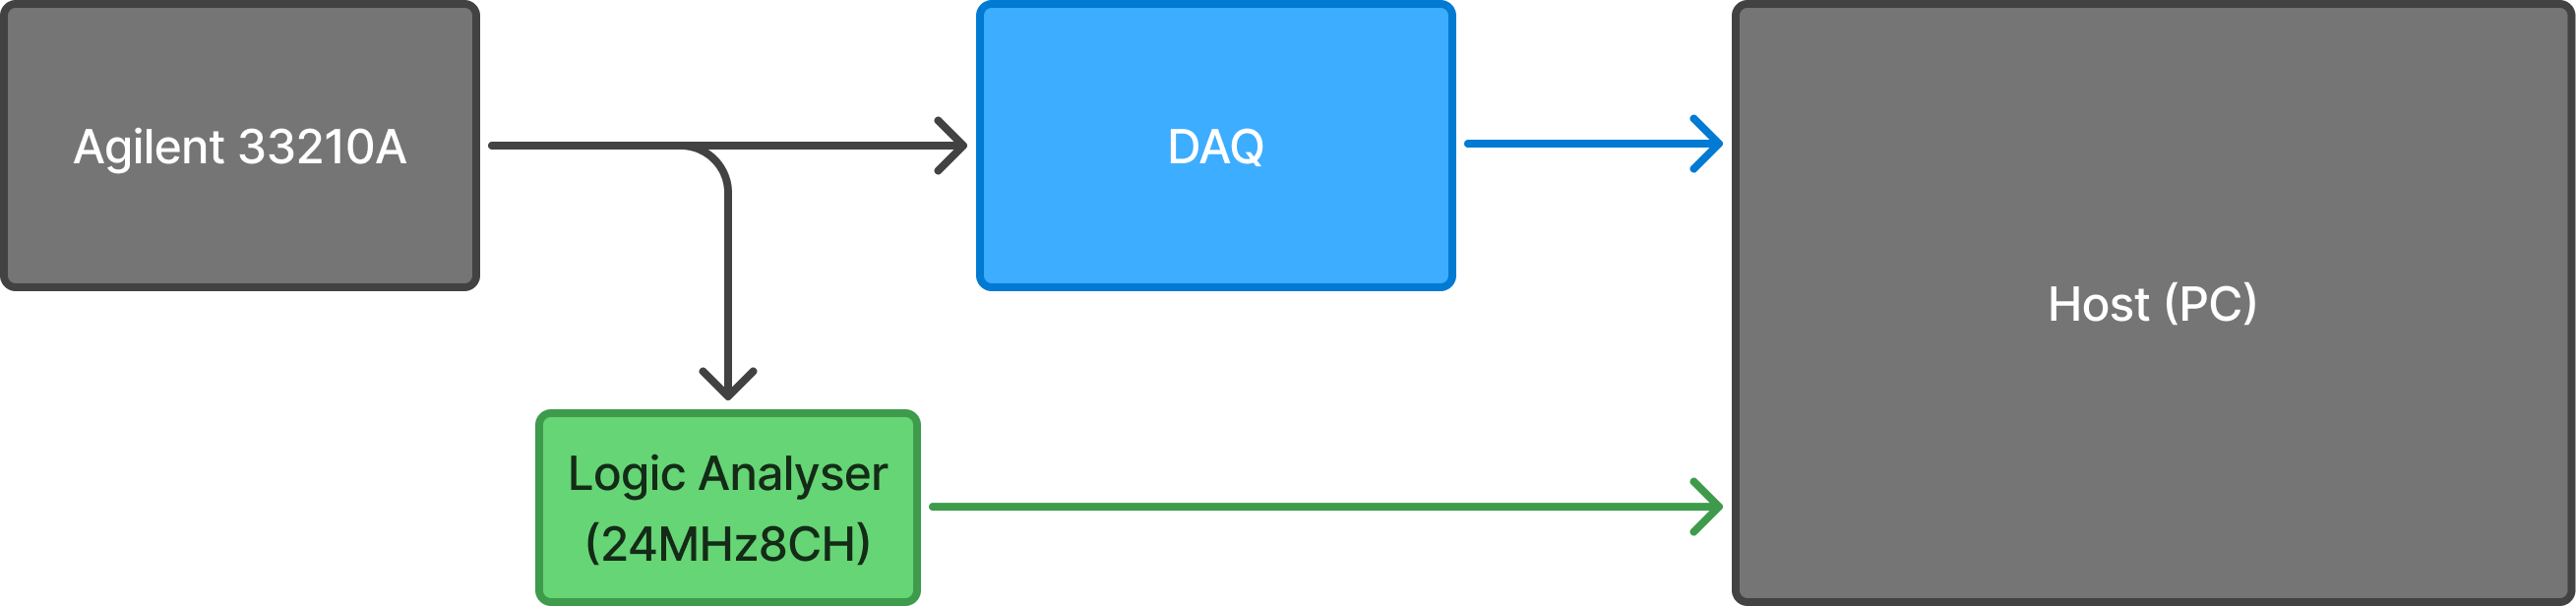
\includegraphics[width=0.45\linewidth]{Cap03/img/bancada_diagrama.png}}
  \hfill
  \subfloat[Montagem física: (A) gerador de funções Agilent 33210A; (B) DAQ baseado no RP2350B; (C) instrumento de referência.\label{fig:img2}]{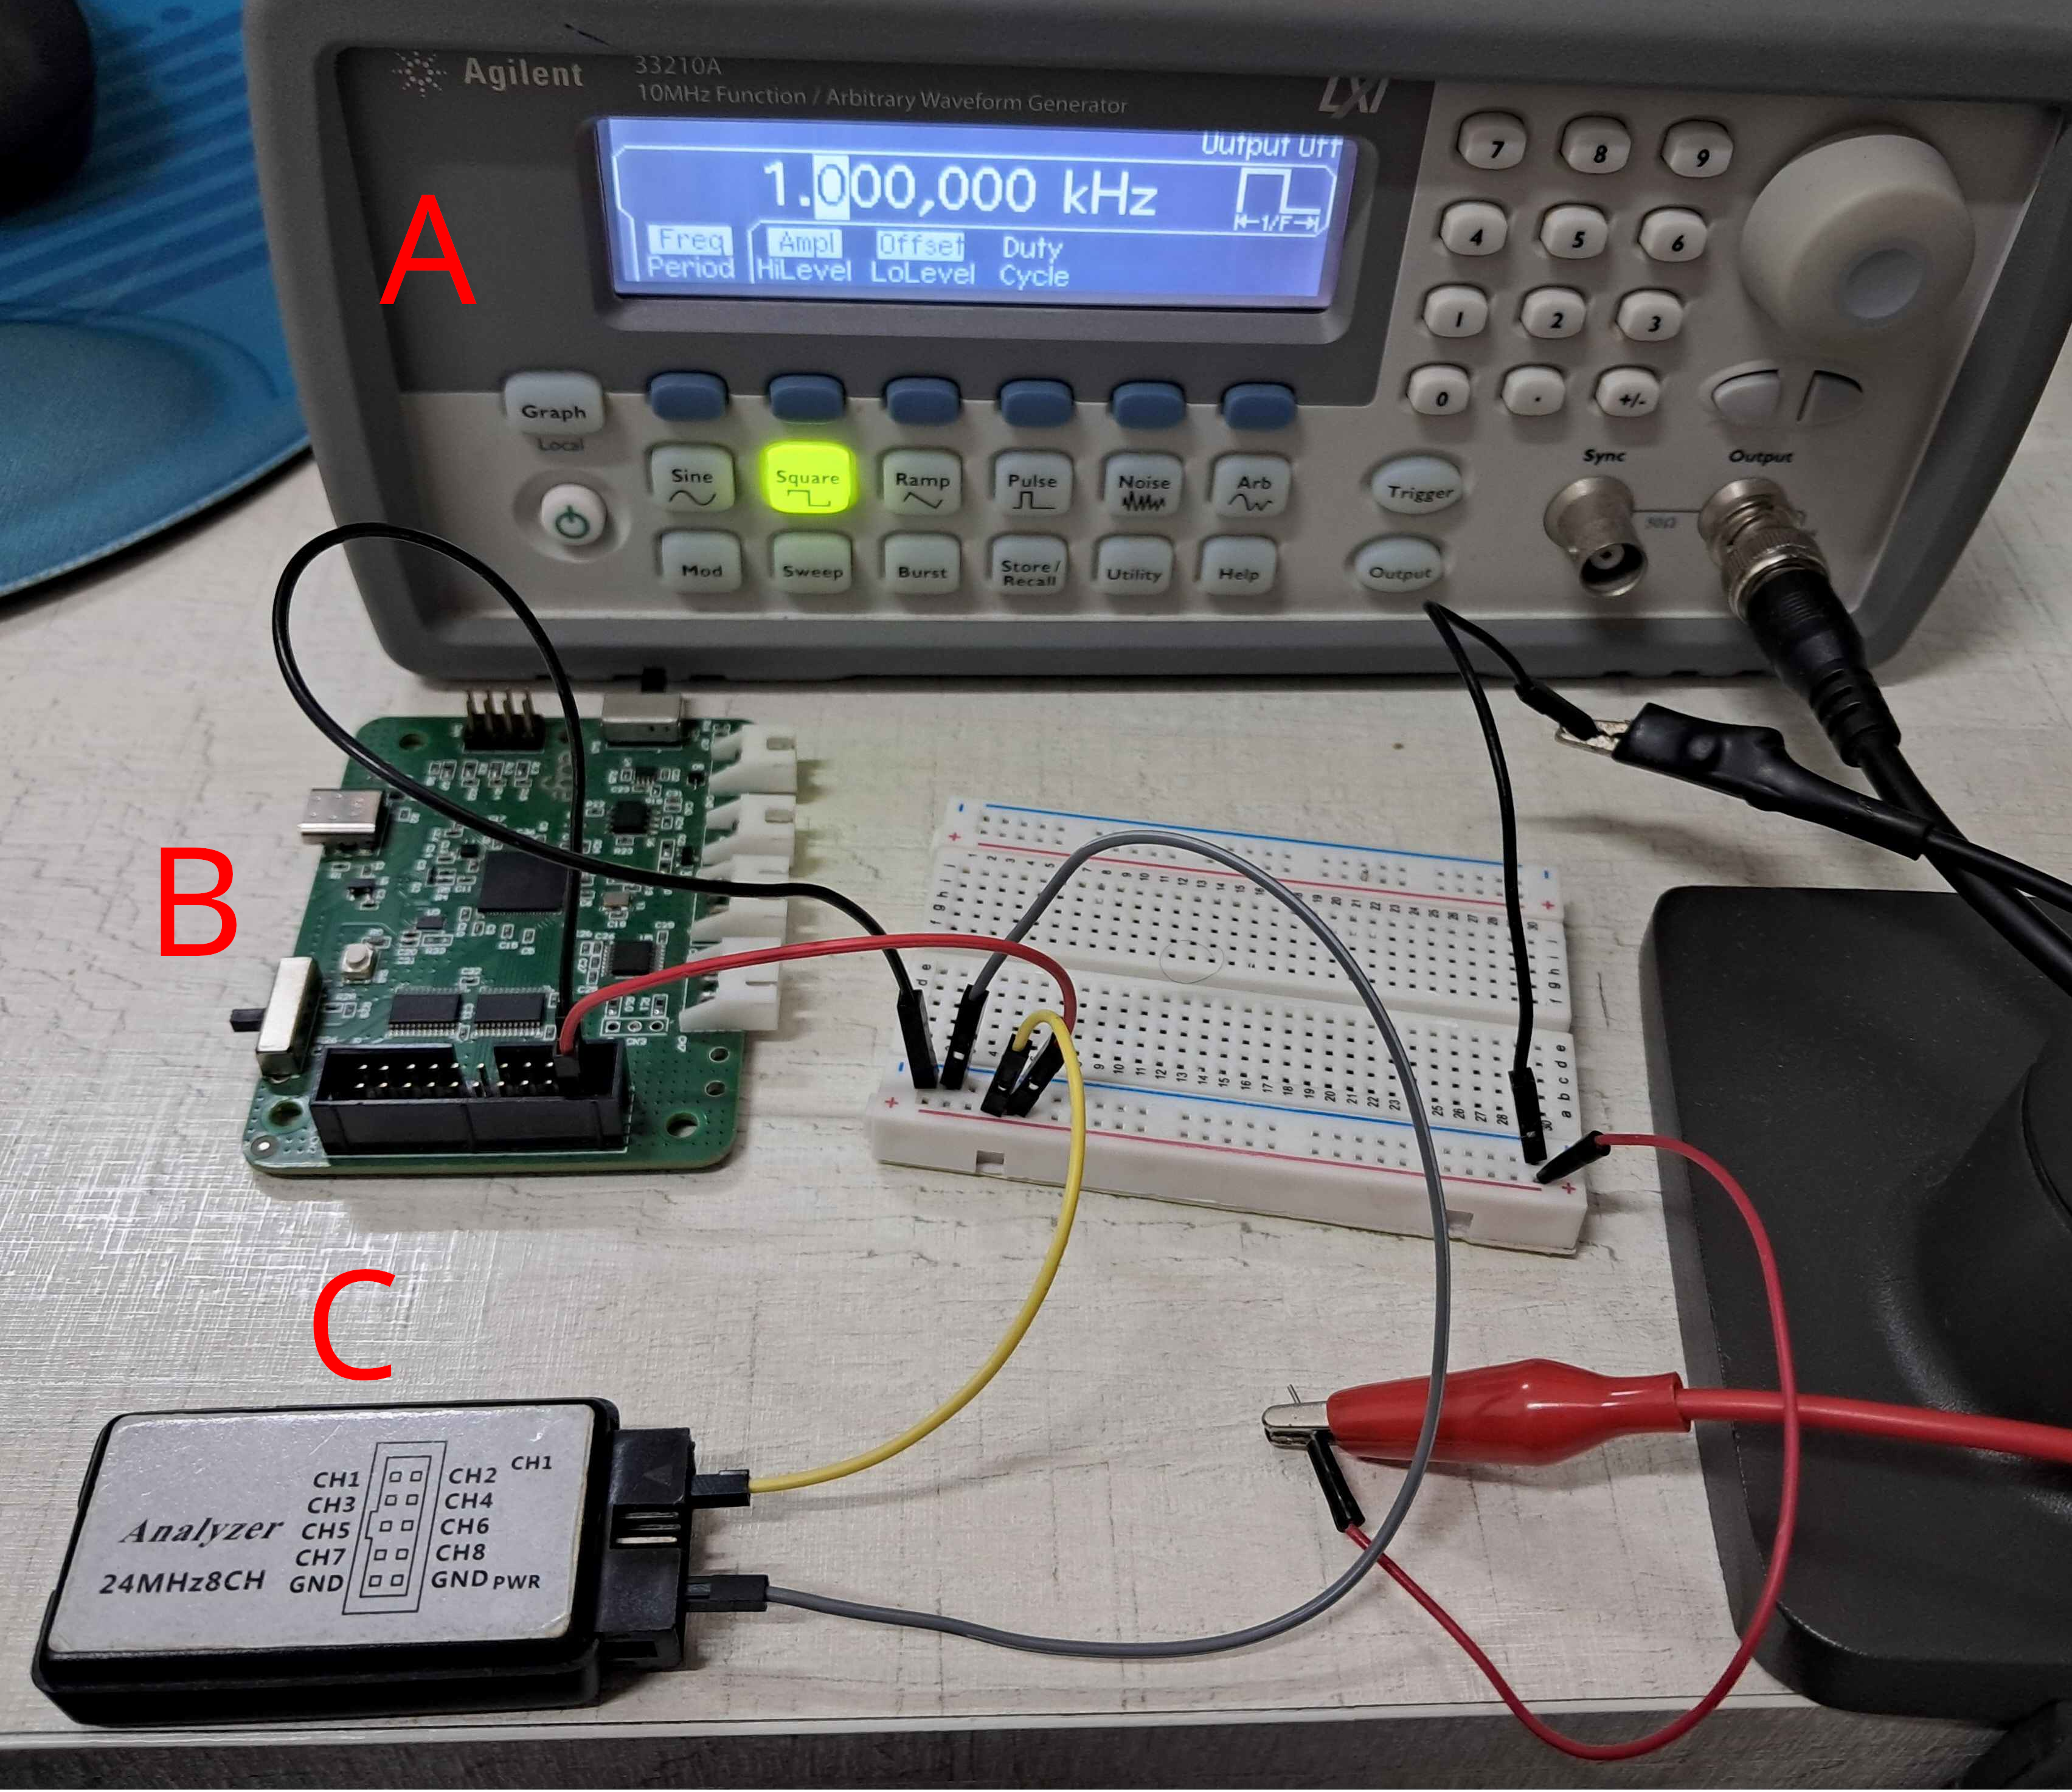
\includegraphics[width=0.45\linewidth]{Cap03/img/bancada_fisica.png}}
  \fonte{Autoria própria.}
\end{figure}

\subsubsection{Placa de aquisição e gerador de sinais}\label{sec:hardware-daq}

A plataforma é o \ac{DAQ}, centrado na RP2350B, com doze canais de
aquisição digital acessíveis por conector de cabo plano de 20 vias (com
tradução de nível para alvos de 1,8\,V a 5,0\,V) e interfaces passivas de
barramento industrial RS-485 e RS-232, não exercitadas nos experimentos, comunicando-se com o \emph{host} por \ac{USB} 2.0
Full Speed.

\begin{figure}[htbp]
  \centering
  \caption{Placa de aquisição (DAQ) baseada no RP2350B.}
  \label{fig:placa-daq}
  \subfloat[Face superior.]{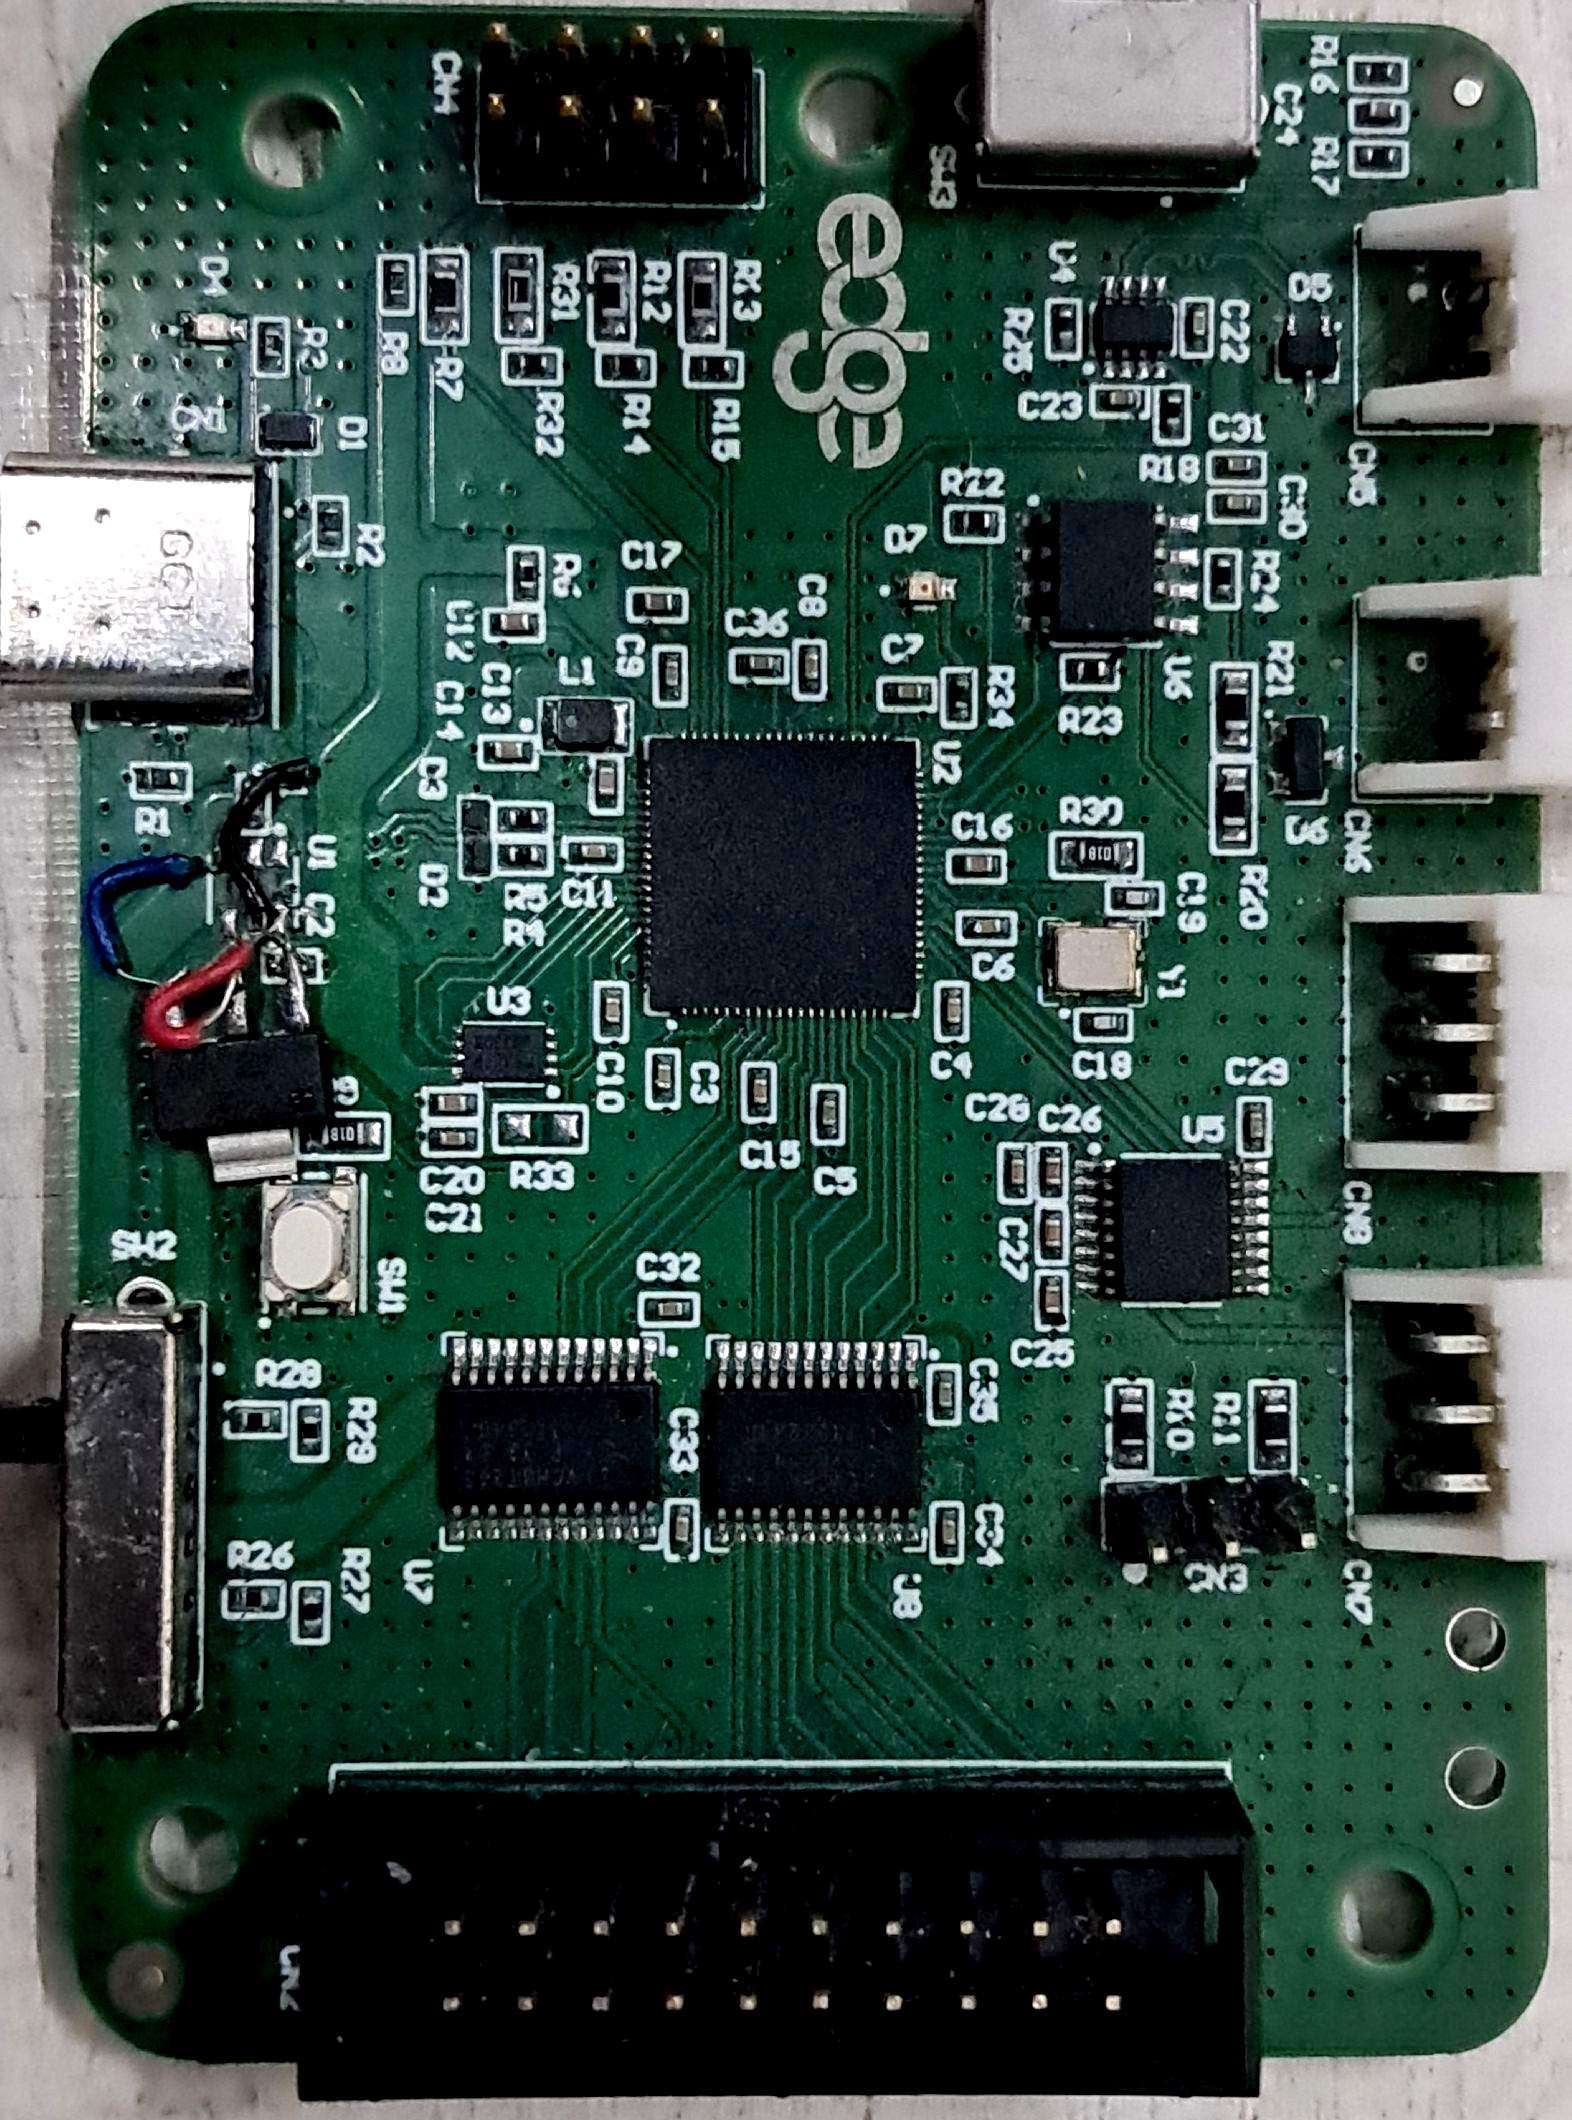
\includegraphics[width=0.45\linewidth]{Cap03/img/placa_daq_top.jpg}}
  \hfill
  \subfloat[Face inferior.]{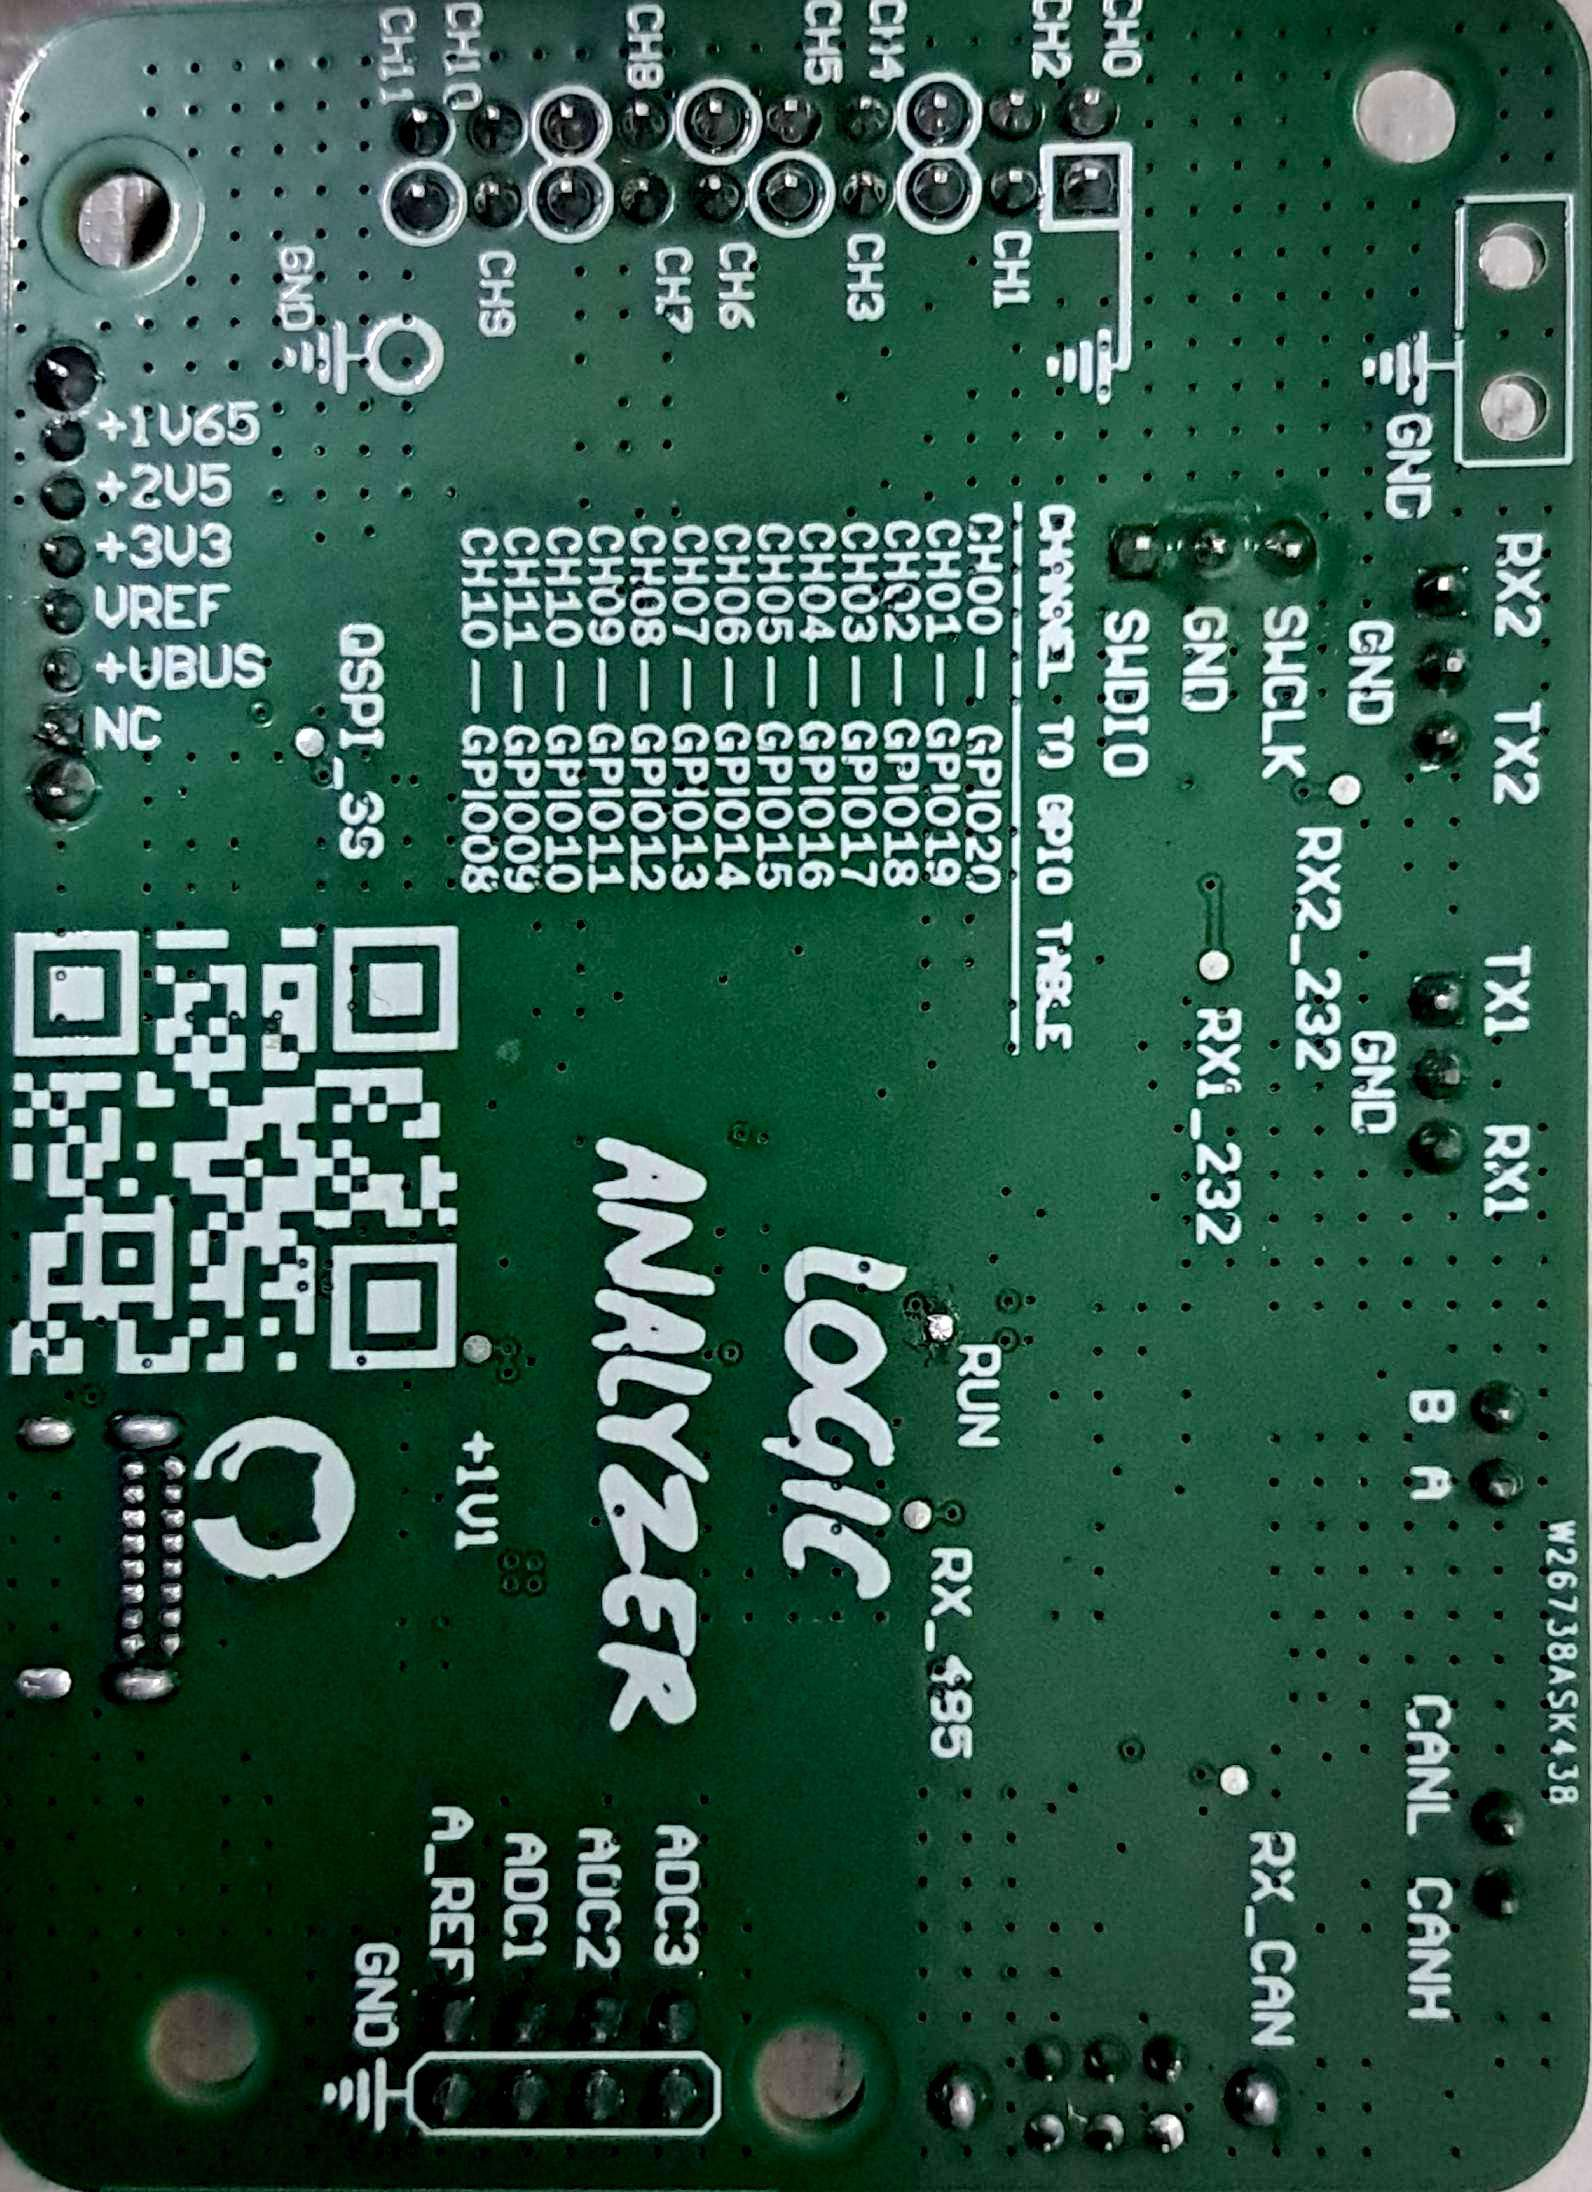
\includegraphics[width=0.45\linewidth]{Cap03/img/placa_daq_bottom.jpg}}
  \fonte{\citeonline{nivuciis_msa}.}
\end{figure}

Em altas velocidades, a integridade física do sinal impõe requisitos ao próprio
hardware de captura: trilhas devem ser tratadas como linhas de transmissão, com
impedância controlada e caminho de retorno de baixa indutância, sob pena de
reflexões e interferência eletromagnética corromperem o sinal antes mesmo da
amostragem \cite{bogatin2011,fan2010,morrison2007}. Esses aspectos foram
observados no projeto da placa utilizada neste trabalho
(Figura~\ref{fig:placa-daq}).

Um gerador de funções Agilent 33210A (até 10\,MHz) produz o sinal de entrada
de todos os ensaios.

\begin{figure}[htbp]
  \centering
  \caption{Gerador de funções Agilent 33210A.}
  \label{fig:gerador-agilent}
  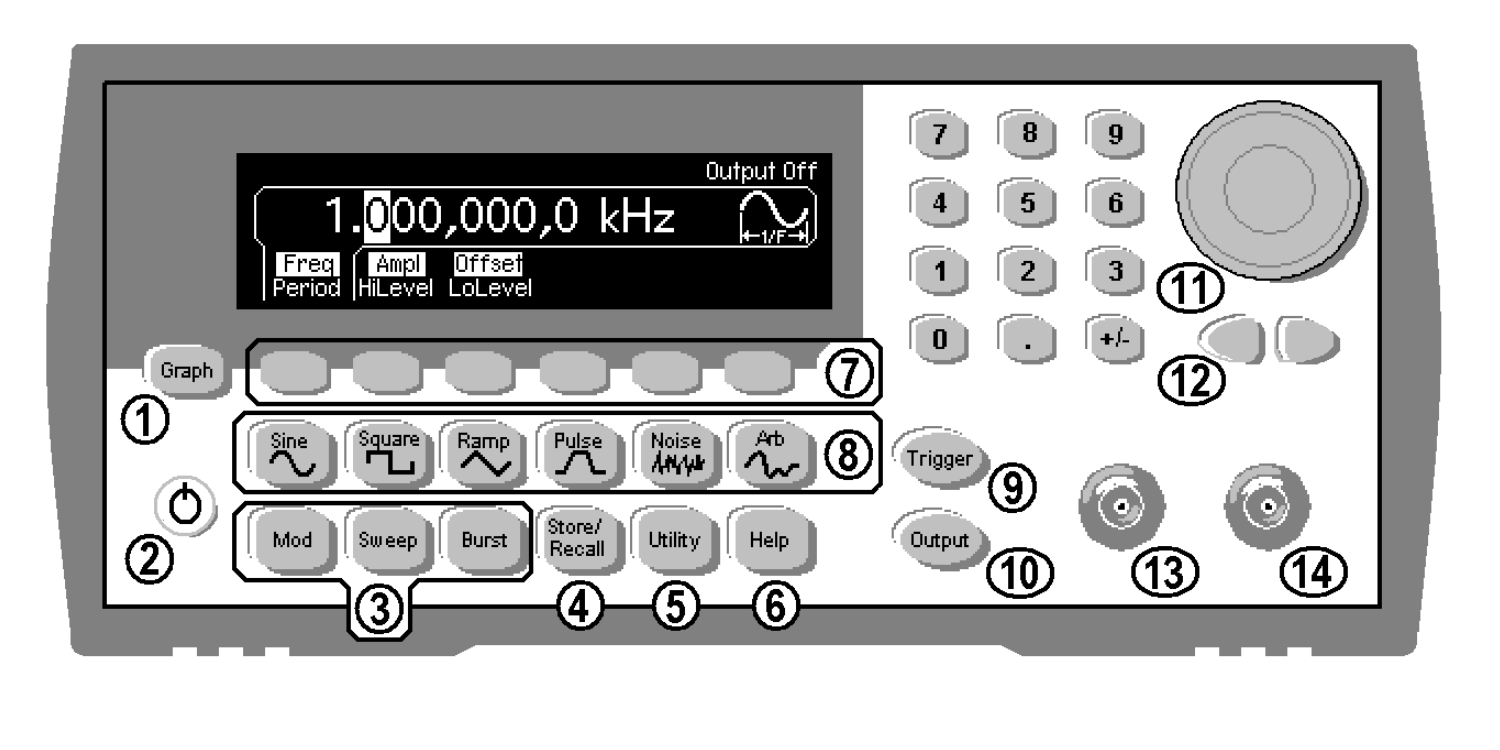
\includegraphics[width=0.5\linewidth]{Cap03/img/gerador_agilent_33210a.png}
  \fonte{adaptado de \citeonline{agilent2008}.}
\end{figure}

Como a banda do \ac{USB} 2.0 Full Speed (12\,Mbit/s) é ordens de grandeza inferior à
taxa de produção de amostras no limite da plataforma, o \ac{RLE}
(Seção~\ref{sec:sigrok-pico}) e o buffer em \ac{SRAM} são componentes essenciais do
caminho de dados em ambas as arquiteturas comparadas \cite{picocoder2023}.

\subsubsection{Instrumentos, \emph{host} e medição}\label{sec:bancada-instrumentos}

\begin{itemize}
  \item \textbf{Gerador de padrões:} o gerador de funções Agilent 33210A (Figura~\ref{fig:gerador-agilent}), configurado para produzir a onda quadrada de 100\,kHz usada em M1, M2 e M3 (em M4, 1\,MHz; ver Seção~\ref{sec:metricas}), aplicada em paralelo ao canal D3 do \ac{DAQ} e ao analisador lógico de referência. A frequência de 100\,kHz foi escolhida porque a compactação \ac{RLE} mantém o fluxo abaixo do teto do \ac{USB} Full-Speed em toda a faixa de taxas varrida; com 1\,MHz, o fluxo quase não se compacta e a medida passa a refletir o barramento, e não o amostrador.

  \item \textbf{Instrumento de referência:} analisador lógico \ac{USB} genérico de 8 canais e 24\,MHz, baseado no microcontrolador Cypress CY7C68013A (FX2LP) e compatível com o \emph{software} da Saleae (Figura~\ref{fig:instrumento-ref}), controlado pelo software Logic~2 (versão 2.4.44) por meio de sua \ac{API} de automação, usado como contador de bordas externo e para aferição da frequência do gerador. A cada repetição, o \emph{script} do \emph{host} arma o \ac{DAQ} e o analisador na mesma borda de subida e compara as duas capturas da mesma janela. Operado a 12\,MS/s, o analisador resolve o tempo em passos de 83,3\,ns, isto é, 120 amostras por período da onda de 100\,kHz, margem suficiente para a contagem de bordas e de períodos frente às taxas do \ac{DAQ} (até $\approx 5$\,MS/s). Sua base de tempo depende de um cristal sem calibração rastreável, o que limita a exatidão absoluta da frequência medida à tolerância desse cristal (tipicamente dezenas de ppm). A medição externa de tempos por um pino de \emph{debug} comutado pelo firmware não foi empregada (Seção~\ref{sec:trabalhos-futuros}); a métrica M4 é medida internamente por \ac{DWT} (item a seguir).

  \begin{figure}[htbp]
    \centering
    \caption{Analisador lógico de referência (FX2LP, 8 canais, 24\,MHz).}
    \label{fig:instrumento-ref}
    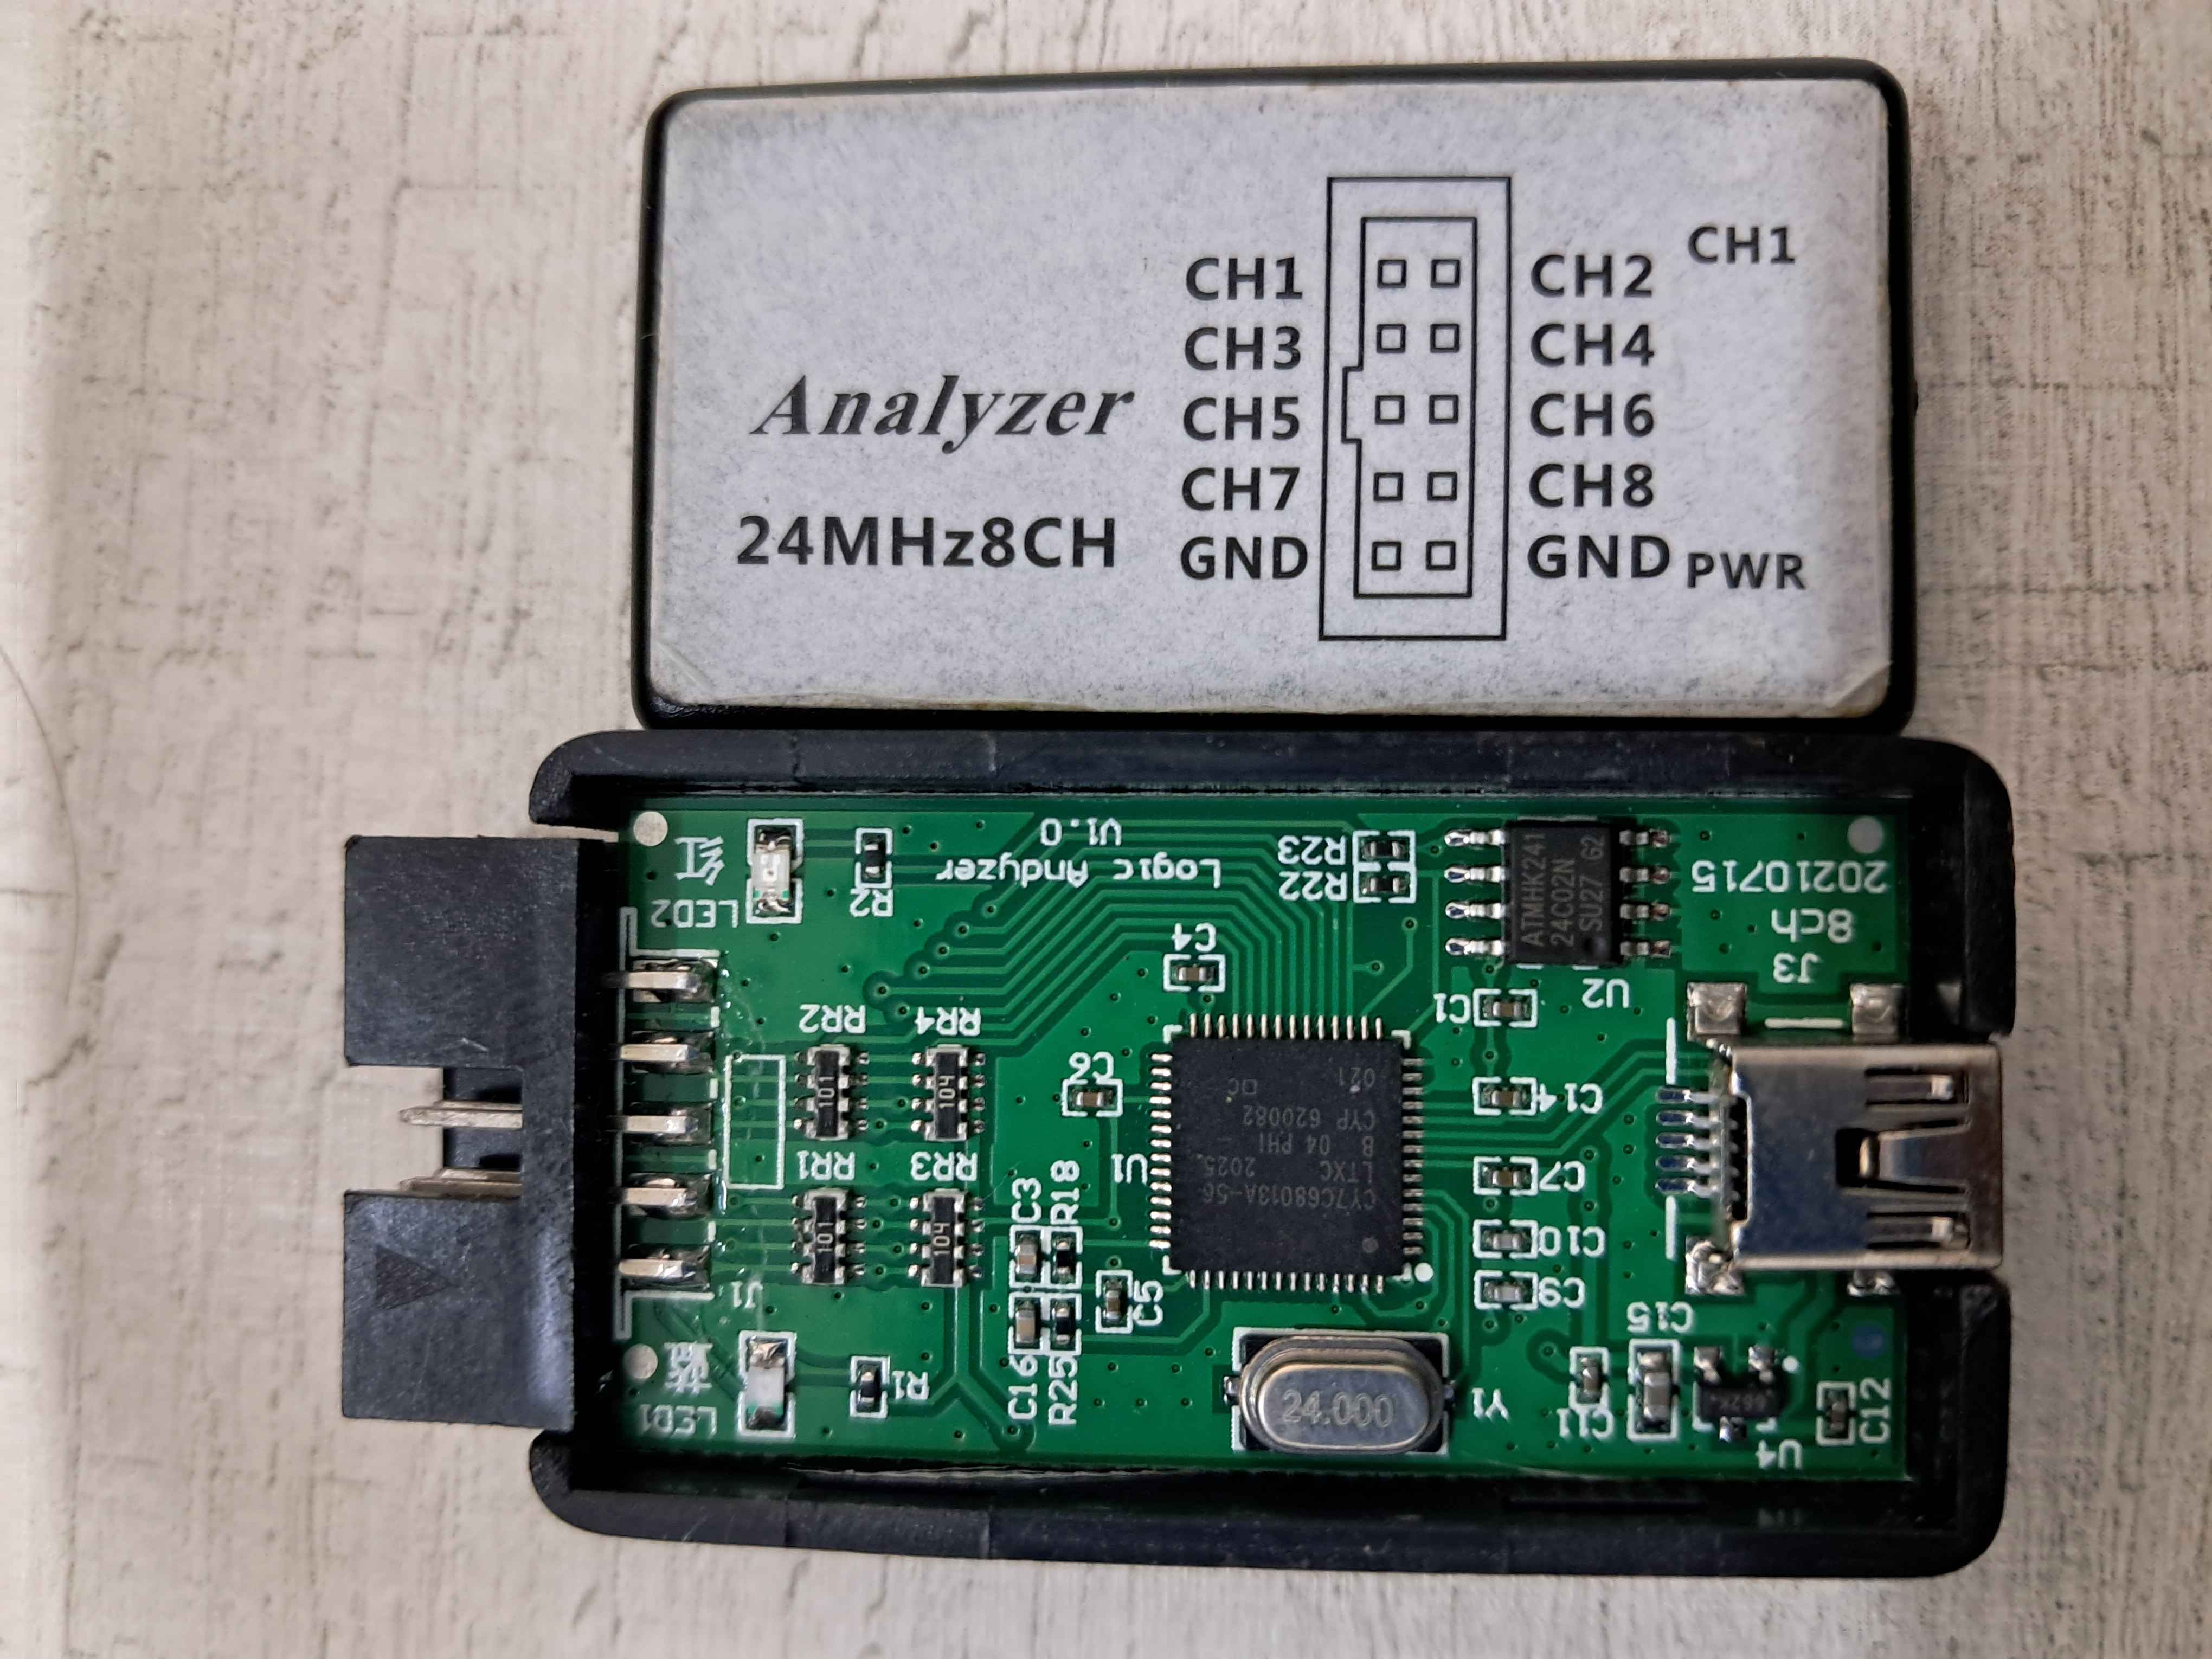
\includegraphics[width=0.5\linewidth]{Cap03/img/intrumento_ref.png}
    \fonte{Autoria própria.}
  \end{figure}

  \item \textbf{Host:} o mesmo computador para todas as medições, com os scripts em \texttt{benchmarks/} (Seção~\ref{sec:metricas}) controlando a captura via protocolo sigrok-pico (repetições, varreduras de taxa); versões fixadas e registradas.

  \item \textbf{Medição interna:} contador de ciclos \ac{DWT} (\texttt{DWT->CYCCNT}) do Cortex-M33 para ciclos por amostra e ocupação de \ac{CPU} \cite{arm2021}, exposto ao \emph{host} por um comando de protocolo dedicado (\texttt{'o'}, fora do conjunto sigrok-pico padrão) consultado por \texttt{benchmarks/m4\_cpu\_occupancy.py}. A perda de amostras não é contada no firmware: é medida no \emph{host}, a partir do fluxo entregue, e o transbordamento da fila de \emph{buffers} de A aparece ao \emph{host} como aborto da captura (\texttt{!!!}).

  \item \textbf{Análise:} scripts Python (diretório \texttt{benchmarks/} do repositório público do trabalho \cite{dias2026artefatos}) para contagem de bordas contra a referência, extração de períodos, histogramas de \emph{jitter} e estatística descritiva, de modo a viabilizar a repetibilidade integral do experimento por terceiros \cite{collberg2016}.
\end{itemize}

Antes das medições finais, a bancada foi validada executando M1 e M3 com
ambos os firmwares e comparando as capturas com a referência. Essa validação
revelou um defeito na primeira versão do Firmware A, que rearmava o \ac{PIO}
e o \ac{DMA} a cada bloco sem sinalizar a lacuna resultante; o defeito foi
corrigido, e todas as medições reportadas no Capítulo~\ref{cap:resultados}
usam a versão corrigida, descrita na Seção~\ref{sec:firmware-a}.

\section{Implementação dos firmwares}\label{sec:firmware}

Ambos os firmwares foram construídos sobre o Pico \ac{SDK}, em C
\emph{bare-metal}, e organizam-se em módulos: \ac{ADC}, captura, abstração de
\ac{PIO}/DMA ou \ac{GPIO}/CPU, protocolos sigrok, interfaces seriais e utilitários \ac{USB}
com \emph{TinyUSB}, distribuída com o \ac{SDK} \cite{rpi2024sdk}. A opção por
firmware \emph{bare-metal}, sem \ac{RTOS}, decorre de a temporização crítica
ser garantida pelo hardware (\ac{PIO}/DMA) e não por um escalonador de tarefas
(Seção~\ref{sec:hardware}); as \acp{API} leves do Pico \ac{SDK} (\texttt{pico\_time},
\texttt{hardware\_*}) oferecem acesso direto aos periféricos com sobrecusto
próximo de zero \cite{rpi2024sdk}. Os dois firmwares implementam o mesmo
conjunto de comandos do protocolo, resumido no Quadro~\ref{qua:comandos}.

\begin{quadro}[H]
  \centering
  \caption{Comandos do protocolo sigrok-pico.}
  \label{qua:comandos}
  \small
  \begin{tabularx}{\linewidth}{|l|>{\raggedright\arraybackslash}X|}
    \hline
    \textbf{Comando} & \textbf{Descrição}                             \\ \hline
    \texttt{i}       & Consulta de identificação                      \\ \hline
    \texttt{R}       & Define a taxa de amostragem (5\,kHz--120\,MHz em A; até $\approx 4{,}05$\,MHz em B) \\ \hline
    \texttt{L}       & Define o número de amostras (1--1.000.000)     \\ \hline
    \texttt{a}       & Consulta a escala do canal analógico           \\ \hline
    \texttt{A}       & Habilita/desabilita canal analógico            \\ \hline
    \texttt{D}       & Habilita/desabilita canal digital              \\ \hline
    \texttt{F}       & Captura de comprimento fixo                    \\ \hline
    \texttt{C}       & Captura contínua                               \\ \hline
    \texttt{t}       & Configura disparo                              \\ \hline
    \texttt{o}       & Consulta a ocupação de \acs{CPU} (extensão deste trabalho) \\ \hline
  \end{tabularx}
  \fonte{Autoria própria.}
\end{quadro}

\subsection{Firmware A (linha de base): aquisição por PIO+DMA}\label{sec:firmware-a}

\begin{figure}[htbp]
  \centering
  \caption{Arquitetura do Firmware A (PIO+DMA).}
  \label{fig:fw-a-arch}
  \vspace{-1cm}
  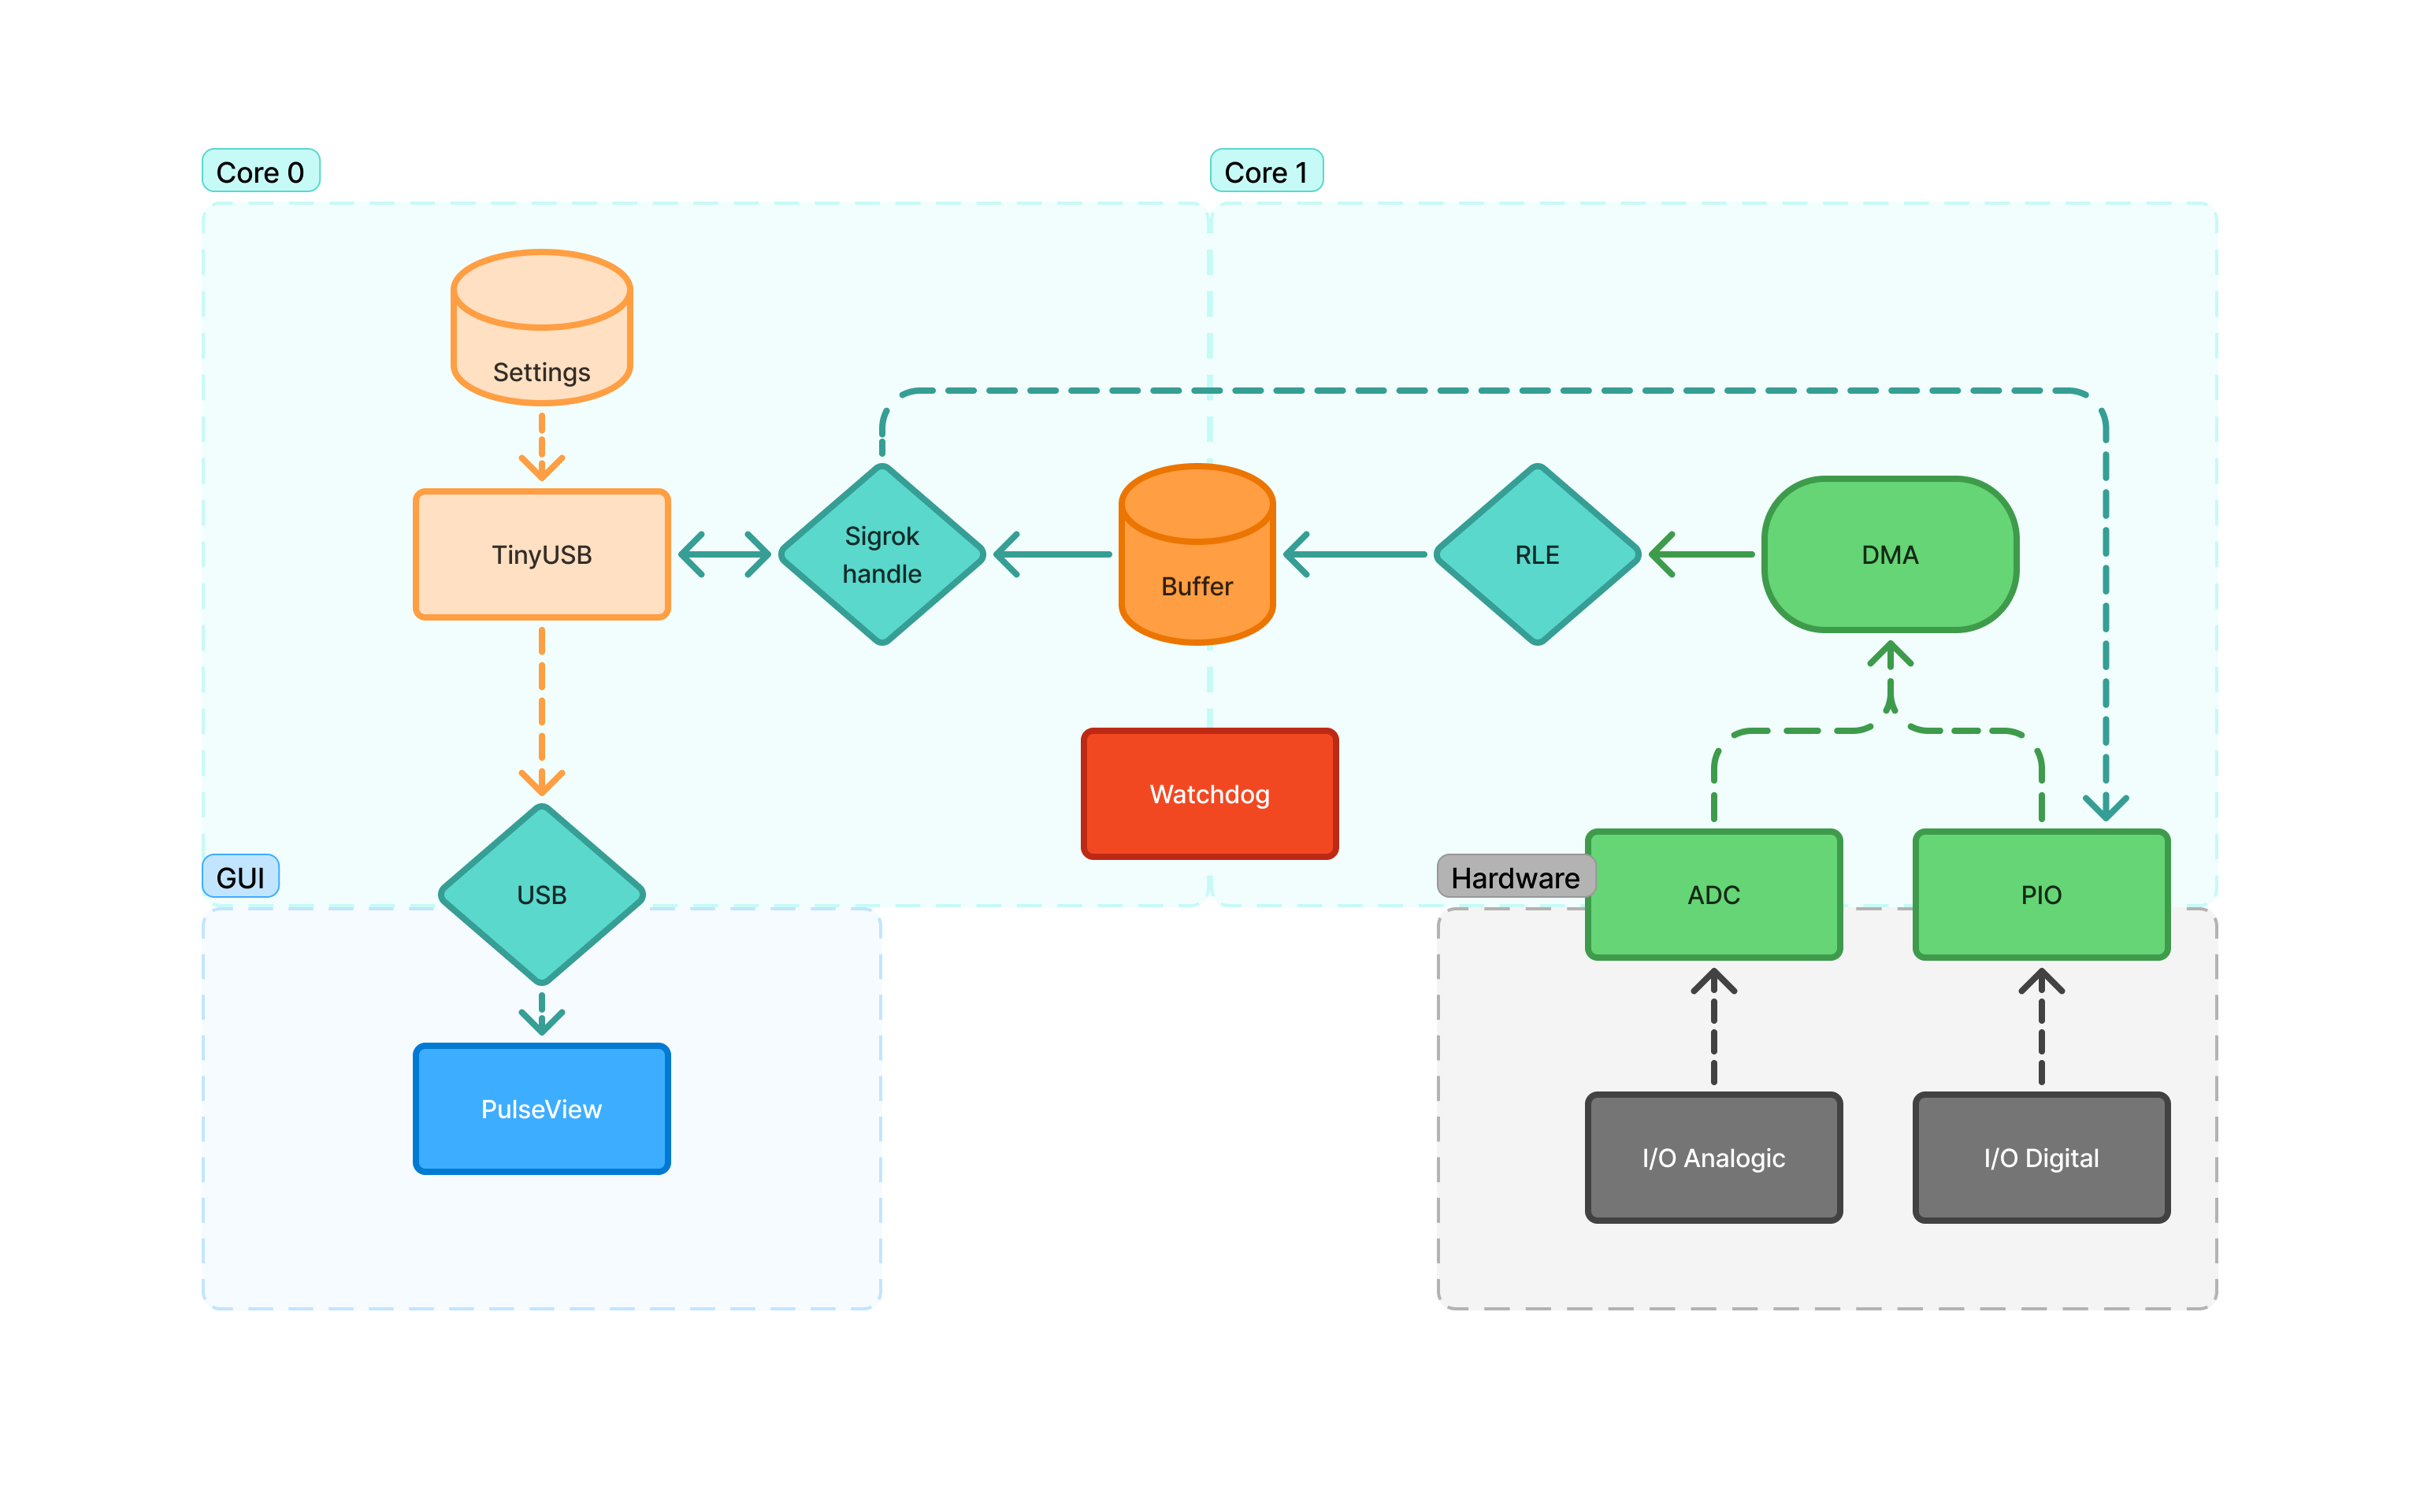
\includegraphics[width=1\linewidth]{Cap03/img/fw_A_arch.png}
  \vspace{-2cm}
  \fonte{Autoria própria.}
\end{figure}

O firmware A (Figura~\ref{fig:fw-a-arch}) implementa a amostragem inteiramente em hardware. Seis variantes
de programa \ac{PIO} são compiladas no binário: a mais simples executa em laço a
instrução \texttt{in pins, 12}, amostrando os doze canais digitais a cada ciclo
do clock da máquina de estados, com \emph{autopush} para o \ac{FIFO} a cada amostra
de 12 bits, que é o caminho de taxa máxima, com \emph{jitter} limitado ao divisor de
clock da máquina de estados (Equação~\ref{eq:clkdiv}). As demais
variantes antepõem ao laço de captura um estágio de espera baseado em
\texttt{jmp pin}, que monitora o \ac{GPIO} de disparo sem custo sobre a temporização
da captura subsequente, implementando disparo assistido por hardware (borda de
subida, borda de descida, qualquer borda, nível alto e nível baixo). Em todos
os casos, a taxa é programada pelo divisor de clock da máquina de estados
(Equação~\ref{eq:clkdiv}), cobrindo o intervalo de 5\,kHz a 120\,MHz exposto ao
\emph{host}.

O transporte das amostras também ocorre sem intervenção da \ac{CPU} no caminho
de cada amostra. Nas capturas apenas digitais, de comprimento fixo
(\texttt{F}) ou contínuas (\texttt{C}) e com ou sem disparo, dois canais de
\ac{DMA}, ritmados pelo \ac{DREQ} do \ac{FIFO} de recepção do \ac{PIO}, transferem as amostras
(unidades de 16 bits) para dois \emph{buffers} de 1\,024 amostras em \ac{SRAM} em
regime de \emph{ping-pong}: cada canal, ao completar seu \emph{buffer},
dispara o outro por encadeamento (\emph{chain}), de modo que a amostragem
nunca para; a interrupção de fim de bloco apenas contabiliza o \emph{buffer}
produzido e verifica se a \ac{CPU} já liberou o anterior. Se a \ac{CPU} ainda não tiver
consumido um \emph{buffer} quando o \ac{DMA} precisar reescrevê-lo, a fila de dois
\emph{buffers} transbordou: o firmware aborta a captura e envia ao \emph{host} o
marcador de erro \texttt{!!!} do protocolo, em vez de descartar amostras em
silêncio. Com disparo, o programa \ac{PIO} espera a condição via \texttt{jmp pin} e
só então entra no mesmo laço de amostragem, de forma que o disparo apenas
determina o início da captura. Na captura contínua, o \ac{DMA} é armado uma única
vez e o fluxo é fatiado nos blocos de $L$ amostras definidos pelo comando
\texttt{L}, cada um encerrado por um marcador com a contagem de \emph{bytes}
do bloco (\texttt{\$n+}), que permite ao \emph{host} verificar a completude. Apenas
as capturas com canais analógicos usam um caminho distinto, em que a \ac{CPU}
rearma o \ac{DMA} a cada bloco; esse caminho não é exercitado nos experimentos.
Em todos os casos, fora do caminho crítico de amostragem, a \ac{CPU} aplica \ac{RLE}
aos \emph{buffers} capturados, em que sequências de até 32 amostras idênticas
consecutivas colapsam em três \emph{bytes}, e os transmite ao \emph{host} via \ac{USB}
\ac{CDC} (TinyUSB).

Durante a captura, portanto, a \ac{CPU} permanece \textbf{fora do caminho de
  amostragem}: em nenhum dos dois modos ela lê os pinos ou conta ciclos por
amostra; seu papel se limita a monitorar \ac{DMA} e conexão \ac{USB} e, entre blocos,
codificar e transmitir os dados já amostrados, abortando a captura se o \emph{host}
desconectar. Essa é a propriedade arquitetural cujo valor este trabalho
quantifica.

\subsection{Firmware B: aquisição por GPIO+CPU}\label{sec:firmware-b}

\begin{figure}[htbp]
  \centering
  \caption{Arquitetura do Firmware B (GPIO+CPU).}
  \label{fig:fw-b-arch}
  \vspace{-1cm}
  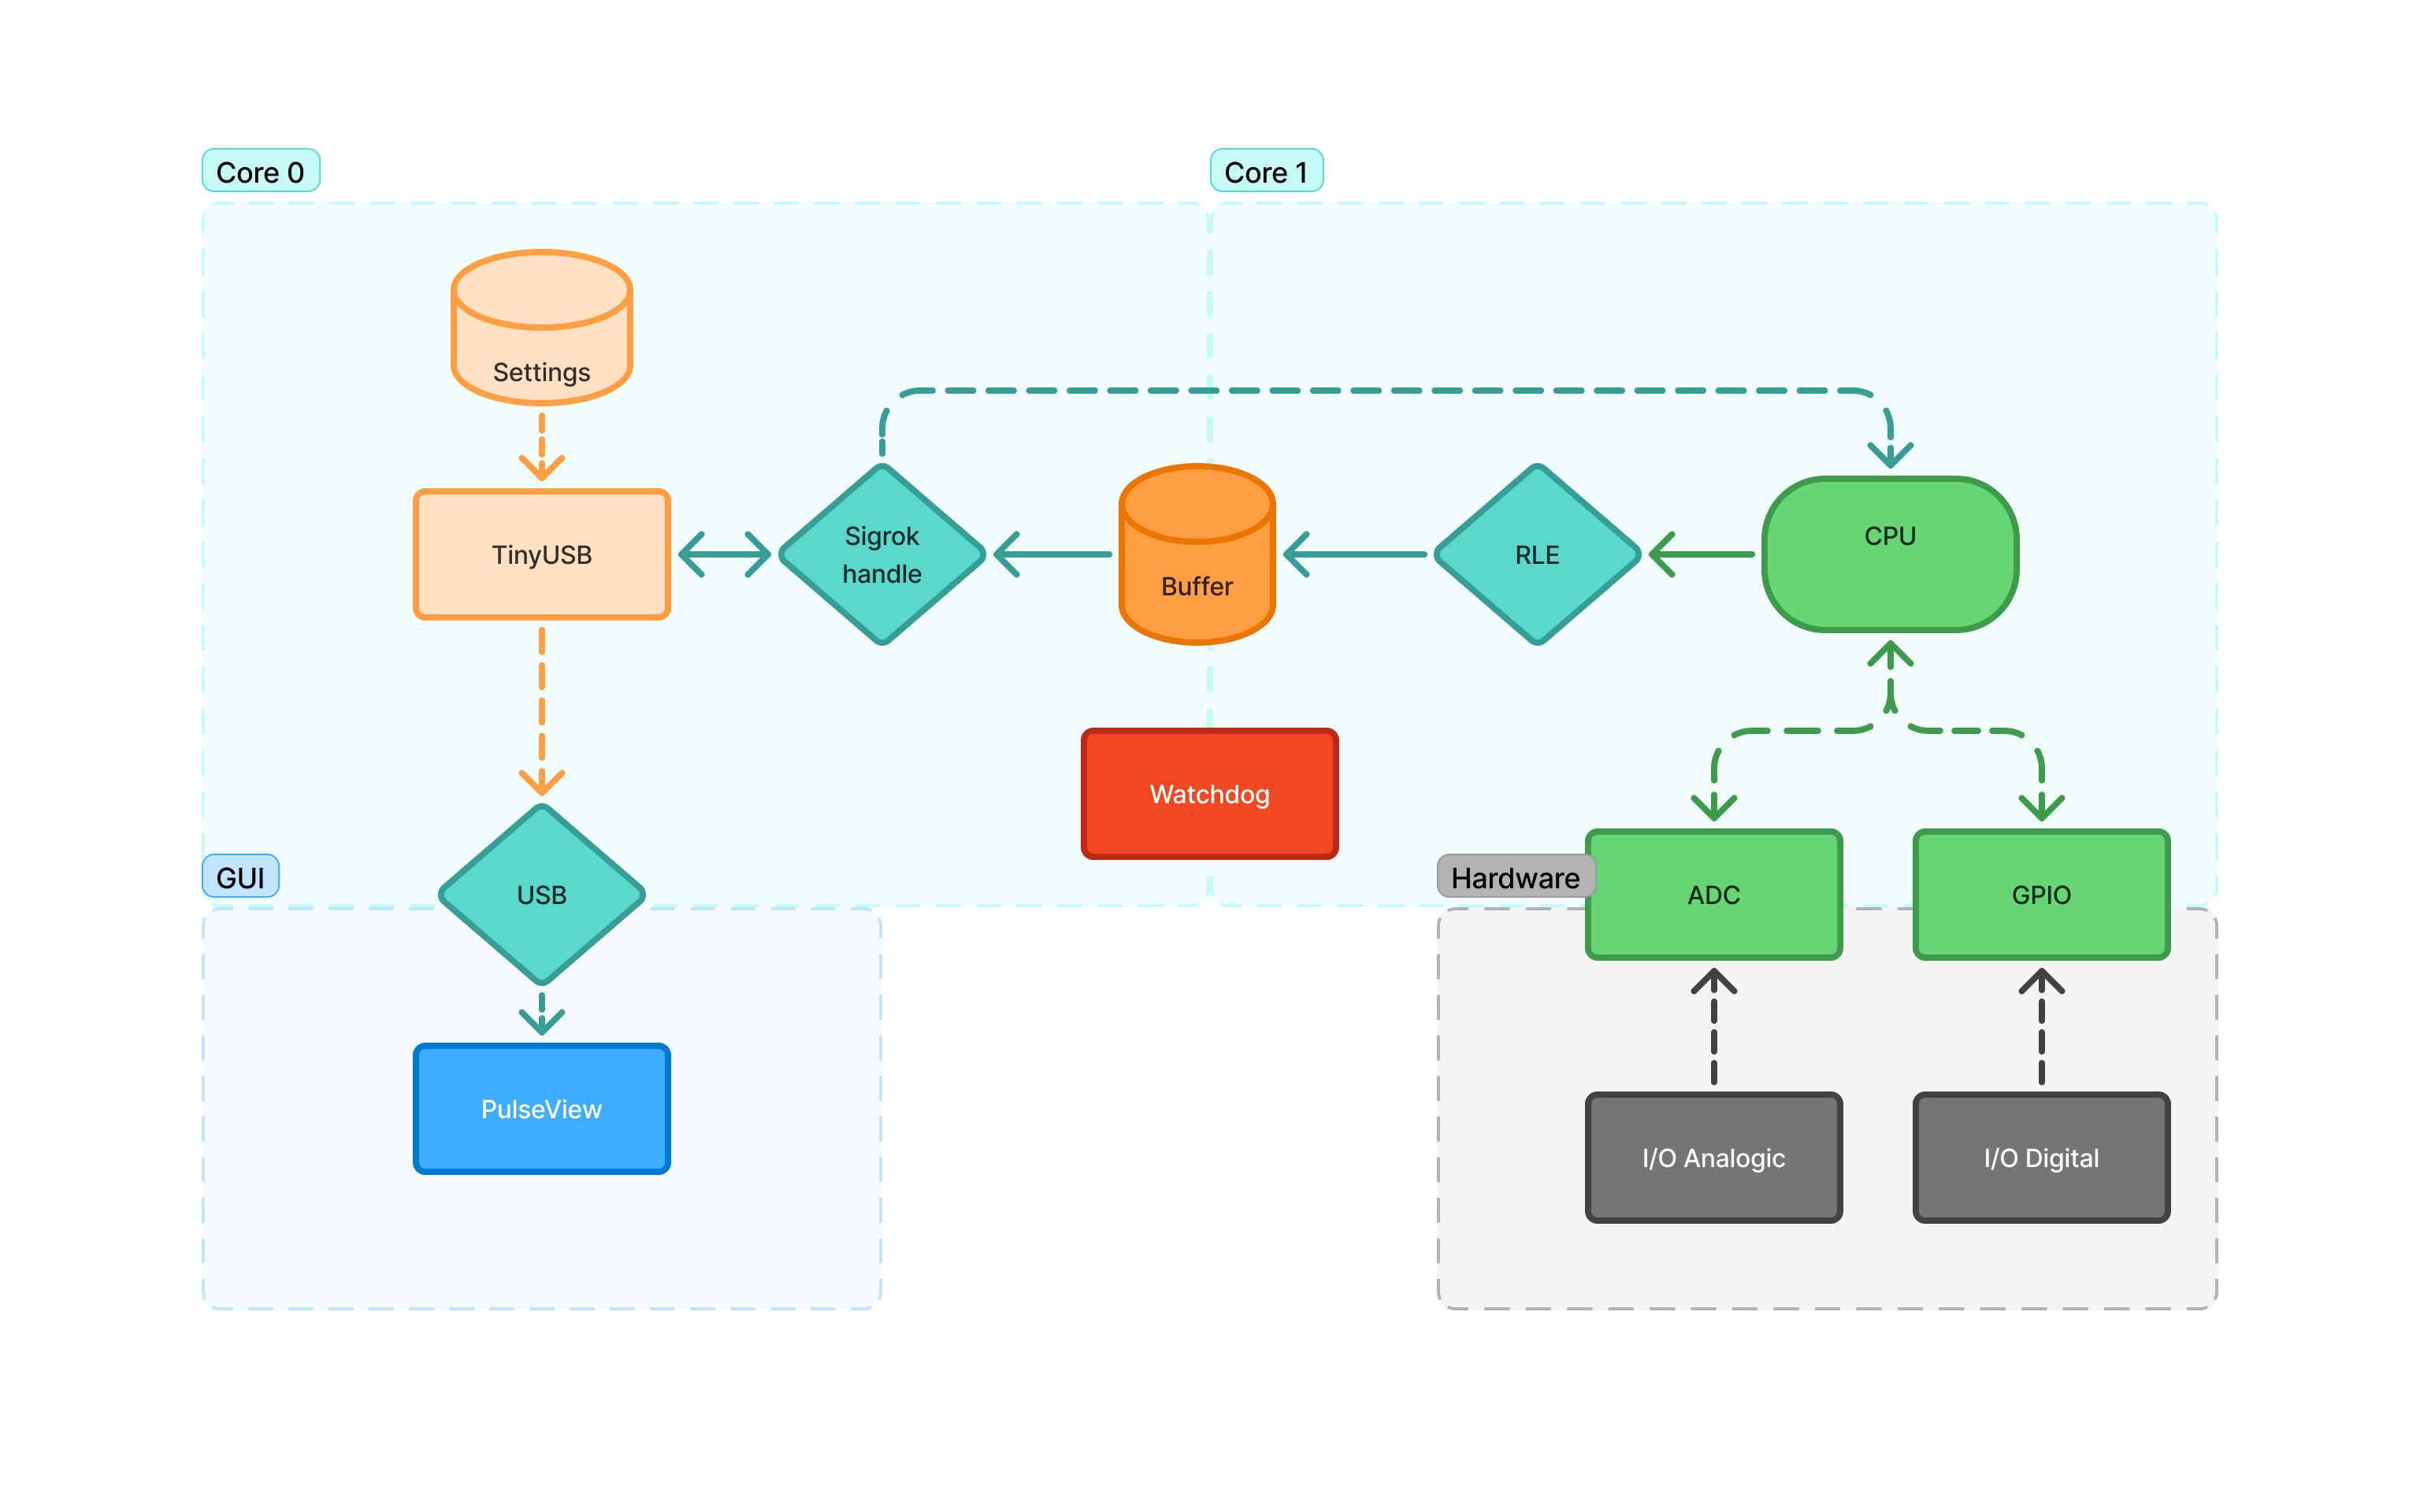
\includegraphics[width=1\linewidth]{Cap03/img/fw_B_arch.png}
  \vspace{-2cm}
  \fonte{Autoria própria.}
\end{figure}

O firmware B (Figura~\ref{fig:fw-b-arch}) substitui os estágios de amostragem e transporte do caminho de
dados por software, mantendo inalterados os estágios de codificação e
transmissão (\ac{RLE}, TinyUSB, protocolo, formato das amostras). As amostras são
obtidas pela leitura do registrador de entrada do bloco \ac{SIO}, no \ac{SDK}
\texttt{gpio\_get\_all()}, que retorna o estado de todos os \acp{GPIO} em uma
única leitura de 32 bits, da qual se extraem os 12 bits dos canais; essa é a
forma mais rápida de leitura de \ac{GPIO} disponível à \ac{CPU} no RP2350. O núcleo do
firmware é um laço apertado que lê o \ac{SIO}, armazena a amostra no buffer e
controla o período pelo contador de ciclos \texttt{CYCCNT} da unidade \ac{DWT}, que conta os
ciclos de $f_{clk}$: cada amostra espera o seu próprio prazo absoluto, obtido
somando o período ao prazo anterior, com a parte fracionária do período
acumulada em ponto fixo para que capturas longas não derivem. Assim, um atraso
eventual do laço atinge apenas a amostra em que ocorre, e as seguintes retomam
a grade de tempo, em vez de alongar todos os períodos. Na inicialização, o
firmware mede o custo de uma iteração do laço ($C_{iter}$) e recusa taxas que
exijam menos ciclos por amostra que esse custo acrescido de uma margem de
5\,\%. O laço é escrito em C e executado a partir da flash (\acs{XIP}), com as
interrupções habilitadas, como em uma aplicação convencional.

Uma variante adicional, prevista no projeto mas não avaliada nos experimentos
deste trabalho, explora os dois núcleos do RP2350: o núcleo 1 executa
exclusivamente o laço de amostragem, escrevendo em um buffer circular em \ac{SRAM},
enquanto o núcleo 0 executa TinyUSB, o protocolo e o \ac{RLE}, consumindo esse
buffer. A sincronização usa índices de escrita/leitura em posições de memória
distintas (produtor único/consumidor único), sem travas no caminho quente, e as
interrupções permanecem desabilitadas no núcleo 1 durante a captura. Todos
os resultados do Capítulo~\ref{cap:resultados} referem-se à variante de núcleo
único, em que o mesmo núcleo amostra, codifica e transmite.

O disparo por borda/nível, por sua vez, é implementado por comparação em
software no próprio laço (leitura, máscara e comparação com o estado anterior),
ao contrário do Firmware A, cujo disparo é assistido por hardware via \ac{PIO}
(Seção~\ref{sec:firmware-a}). Fora esses pontos, nada muda em relação ao
Firmware A: protocolo sigrok-pico, \ac{RLE}, TinyUSB e seus \emph{buffers}, clock do
sistema e placa são idênticos, e mudam apenas os mecanismos de amostragem e
transporte e, em consequência deles, o tamanho do par de \emph{buffers} de
amostras digitais: 1\,024 amostras cada no Firmware A e 8\,192 no Firmware B.
No Firmware B, a \ac{CPU} não amostra enquanto codifica e envia um bloco, de modo
que cada fronteira de bloco é uma pausa na amostragem; blocos maiores reduzem o
número dessas pausas e, portanto, favorecem o Firmware B na comparação. No
Firmware A, em que o \ac{DMA} continua amostrando durante o envio, o tamanho
original do projeto foi mantido. O firmware B é desenvolvido em \emph{branch}
dedicado do mesmo repositório, a partir do mesmo \emph{commit} base do firmware
A, com rastreabilidade por \emph{tag}.

\subsection{Ocupação de memória dos firmwares}\label{sec:fw-memoria}

A Tabela~\ref{tab:fw-memoria} compara o tamanho dos dois binários, obtido das
seções do arquivo \ac{ELF} gerado na compilação, em relação à flash de 2\,MB
declarada para a placa e aos 512\,KB de \ac{SRAM} principal do RP2350. A
diferença entre as duas versões concentra-se na seção de dados não
inicializados (\ac{BSS}), que abriga os \emph{buffers} de amostras.

\begin{table}[H]
  \centering
  \caption{Ocupação de memória dos Firmwares A e B.}
  \label{tab:fw-memoria}
  \begin{tabular}{@{}lrrr@{}}
    \toprule
    \textbf{Seção}                 & \textbf{Firmware A} & \textbf{Firmware B} & \textbf{B $-$ A} \\
    \midrule
    Código e constantes (flash)    & 51,7\,KB            & 46,2\,KB            & $-5{,}5$\,KB     \\
    Dados não inicializados (\acs{BSS})  & 109,2\,KB           & 225,3\,KB           & $+116{,}1$\,KB   \\
    \midrule
    Ocupação da flash (2\,MB)      & 2,5\,\%             & 2,3\,\%             & ---              \\
    Ocupação da \acs{SRAM} (512\,KB)     & 21,3\,\%            & 44,0\,\%            & ---              \\
    \bottomrule
  \end{tabular}
  \fonte{Autoria própria.}
  \nota{nenhum dos binários possui dados inicializados (\texttt{.data}) relevantes; 1\,KB = 1\,024 \emph{bytes}.}
\end{table}

Os dois binários ocupam uma fração pequena da flash. O Firmware A é 5,5\,KB
maior por embutir as seis variantes de programa \ac{PIO} e o código de configuração
e encadeamento do \ac{DMA}, que o Firmware B substitui por um laço único em C. Na
\ac{SRAM}, a relação se inverte: o Firmware B ocupa o dobro. Toda a diferença vem
dos \emph{buffers}: a constante de tamanho de bloco, elevada de 1\,024 para
8\,192 amostras, é compartilhada pelos pares de \emph{buffers} dos módulos
digital, RS-232 e RS-485 (seis \emph{buffers} de 2\,KB passam a 16\,KB, ou
84\,KB a mais), e o disparo por software de B mantém um histórico circular de
8\,192 palavras de 32 bits para as amostras de pré-disparo (32\,KB), que em A
é dispensado pelo disparo assistido pelo \ac{PIO}. As estruturas do TinyUSB e o
anel de transmissão \ac{USB} são idênticos nos dois. Mesmo com 44\,\% da \ac{SRAM}, o
Firmware B ainda cabe com folga no RP2350; o custo de memória, portanto, não
restringe a comparação, mas indica que a compensação adotada para B (blocos
maiores para reduzir as pausas de amostragem) é paga em \ac{SRAM}, recurso que o
Firmware A preserva.

\section{Métricas e procedimentos experimentais}\label{sec:metricas}

As métricas adotadas são quatro, definidas antes da coleta: taxa de amostragem máxima
sustentada, \emph{jitter} de amostragem, taxa de perda de amostras e ocupação
de \ac{CPU}. Restringir o conjunto a essas quatro grandezas, previamente definidas e
não selecionadas \emph{a posteriori}, evita diluir o orçamento experimental
(réplicas, tempo de bancada) em comparações que não sustentam o objetivo
geral do trabalho e reduz o risco de \emph{garden of forking paths} na análise
\cite{georges2007,mytkowicz2009}.

Cada métrica é executada com $N = 30$ repetições por ponto de medição, tamanho
amostral escolhido, conforme detalhado na Seção~\ref{sec:analise-estatistica},
por equilibrar a precisão dos intervalos de confiança e o tempo de bancada,
seguindo a prática de repetir as execuções e reportar a variabilidade
observada em vez de medições isoladas \cite{georges2007,kalibera2013},
reportando-se as estatísticas descritas
na Seção~\ref{sec:analise-estatistica}. Salvo indicação, varre-se a taxa de amostragem em passos logarítmicos
dentro da faixa suportada, interrompendo a varredura de cada firmware e
contagem de canais na primeira taxa em que o critério da métrica falha em
todas as repetições ou que o firmware recusa na configuração. Em M1, M2 e M3, o sinal é aplicado ao canal D3, e a
varredura é repetida com 4 e com 12 canais habilitados, contagens que
exercitam, respectivamente, um e dois \emph{bytes} por amostra no protocolo; em
M4, usam-se 1, 8 e 12 canais, com a onda de 1\,MHz aplicada aos canais, sinal
com muitas transições que exercita o custo da codificação \ac{RLE}, em capturas
curtas de 65\,536 amostras sem disparo, para que a medida reflita o custo de
processamento por amostra, e não o regime sustentado do \ac{USB}.

\paragraph{M1: Taxa máxima de amostragem sustentada.} A onda quadrada do gerador é aplicada ao canal D3 e ao
analisador lógico de referência, que fornece a contagem de bordas de
referência. Em taxa crescente, cada repetição arma um disparo por borda de
subida e mantém a janela de 0,2\,s seguinte. Enquanto a janela cabe no limite
de $10^6$ amostras do protocolo (até 3,66\,MS/s), a captura usa o modo de
quantidade fixa (\texttt{F}); acima disso, como em 5,39\,MS/s, o \emph{script}
usa o modo contínuo (\texttt{C}) armado na mesma borda e corta a janela no
\emph{host}. O \emph{script} do \emph{host} conta as bordas de subida no canal do
sinal. Sendo $n_{DAQ}$ o número de bordas contadas pelo \ac{DAQ} e $n_{ref}$
o contado pela referência na mesma janela, uma repetição é íntegra quando
(i) a janela inteira foi entregue sem erros de decodificação e sem aborto do
firmware e (ii)
\begin{equation}\label{eq:m1-integra}
  \left| n_{DAQ} - n_{ref} \right| \le \max\left(1;\ 0{,}001\, n_{ref}\right),
\end{equation}
isto é, a contagem coincide com a da referência dentro de 0,1\,\%, tolerância
que absorve a diferença entre a taxa solicitada e a efetivamente obtida. Taxas inferiores a
quatro amostras por período do sinal são excluídas, pois a subamostragem altera
a contagem sem representar falha de aquisição. A taxa máxima sustentada é a
maior taxa em que todas as $N$ repetições são íntegras:
\begin{equation}\label{eq:m1-fmax}
  f_{s,\mathrm{sust}} = \max \left\{ f_s \;:\; \text{as } N \text{ repetições em } f_s \text{ satisfazem a Equação~\ref{eq:m1-integra}} \right\}.
\end{equation} Como análise de sensibilidade
secundária, repete-se a mesma classificação com tolerância de $\pm 2$ bordas,
o mínimo que absorve o corte da janela, para verificar se a conclusão
depende da tolerância escolhida. Comparam-se A e B, e o
resultado de B é confrontado com o teto teórico $f_{clk}/C_{iter}$
(Equação~\ref{eq:fsmax}), com $C_{iter}$ medido por \ac{DWT}.

\paragraph{M2: \emph{Jitter} de amostragem.} Captura, com disparo e janela de 0,2\,s, da onda quadrada de
100\,kHz (frequência aferida pelo instrumento de referência), em taxas de 2,0 a
4,05\,MS/s, e análise da distribuição dos períodos medidos entre bordas de
subida consecutivas. Sendo $i_k$ o índice da $k$-ésima borda de subida e
$T_s = 1/f_s$ o período de amostragem, o $k$-ésimo período medido é
\begin{equation}\label{eq:m2-periodo}
  \tau_k = (i_{k+1} - i_k)\, T_s ,
\end{equation}
e reportam-se, por taxa e por firmware, o desvio-padrão $\sigma$ e o valor
pico a pico $\max_k \tau_k - \min_k \tau_k$ dos períodos da janela.

Como o período do sinal raramente é múltiplo inteiro de $T_s$, o intervalo
entre bordas alterna entre $\lfloor P \rfloor$ e $\lceil P \rceil$ amostras,
com $P = f_s/f_{sig}$. Mesmo um amostrador ideal apresenta, portanto, um
desvio-padrão de quantização
\begin{equation}\label{eq:jitter-quant}
  \sigma_q = T_s \sqrt{\varphi\,(1-\varphi)}, \qquad \varphi = P - \lfloor P \rfloor ,
\end{equation}
e apenas o excedente
\begin{equation}\label{eq:jitter-exc}
  \sigma_{exc} = \sqrt{\sigma^2 - \sigma_q^2}
\end{equation}
pode ser atribuído à instabilidade do instante de amostragem. Como $\varphi$
depende da razão exata entre $f_s$ e $f_{sig}$, $\sigma_q$ varia de forma não
monotônica com a taxa. A mesma captura fornece ainda a diferença
$\Delta n = n_{DAQ} - n_{ref}$ entre os números de períodos contados pelo
\ac{DAQ} e pela referência.

\paragraph{M3: Captura contínua e perda de amostras.} Captura contínua (\texttt{C}) da onda quadrada de 100\,kHz com transmissão
simultânea ao \emph{host} por $T = 60$\,s, em taxas a partir de 1,09\,MS/s (abaixo
dela, o período tem menos de oito amostras e a detecção de lacunas perde
sensibilidade). A medida principal é a fração entregue
\begin{equation}\label{eq:m3-fracao}
  \eta = \frac{N_{ent}}{f_s \, T},
\end{equation}
em que $N_{ent}$ é o número de amostras recebidas pelo \emph{host}. Registram-se
também a taxa efetiva, os abortos sinalizados pelo firmware e o número de
lacunas, detectadas quando o intervalo entre bordas consecutivas se afasta do
período nominal $P = f_s/f_{sig}$, em amostras, por mais de 1,5 amostra:
\begin{equation}\label{eq:m3-lacuna}
  \left| (i_{k+1} - i_k) - P \right| > 1{,}5 .
\end{equation} Como o sinal é
periódico, uma lacuna que dure um número inteiro de períodos não é detectada
pelo intervalo entre bordas; a fração entregue é, por isso, a medida principal
de perda, e o número de lacunas, um limite inferior. Este é o experimento que
expõe o conflito amostragem$\times$\ac{USB}.

Como ensaio auxiliar, para separar o limite do barramento do limite do
firmware, mede-se também a vazão \ac{USB} em captura contínua com sinal pouco
compressível (onda de 1\,MHz), de 0,5 a 4\,MS/s, com 4 e 12 canais, em
capturas de 5\,s com três repetições por condição. O \emph{host} registra os
\emph{bytes} recebidos por segundo e a fração de amostras entregue. Por ter
caráter apenas descritivo, esse ensaio não entra na análise estatística.

\paragraph{M4: Ocupação de CPU.} Mede-se, via contador de ciclos \ac{DWT} (\texttt{DWT->CYCCNT}), a fração de ciclos
que a \ac{CPU} permanece ocupada durante a captura, em cada taxa e contagem de
canais:
\begin{equation}\label{eq:m4-ocupacao}
  O = \frac{C_{ocup}}{C_{total}},
\end{equation}
em que $C_{total}$ é o número de ciclos decorridos na captura e $C_{ocup}$, o
número de ciclos contados como ocupados. O que conta como ocupado difere entre os firmwares e decorre da
própria arquitetura: no Firmware A, contam-se apenas os trechos de
codificação \ac{RLE} e transmissão de cada \emph{buffer}, e não a espera pela
\ac{DMA}, já que nela a \ac{CPU} estaria livre para outra tarefa; no Firmware B,
conta-se a captura inteira, porque a \ac{CPU} está no caminho de cada amostra.
Espera-se, em A, ocupação baixa, limitada ao custo de codificar e transmitir
e crescente com a taxa; em B, ocupação próxima de 100\,\% em qualquer taxa. Esta é a métrica que
quantifica diretamente a propriedade arquitetural central do trabalho, isto é, a \ac{CPU}
permanecer ou não fora do caminho de dados (Seção~\ref{sec:firmware-a}).

\section{Análise estatística}\label{sec:analise-estatistica}

Para cada uma das quatro métricas (M1--M4), em cada condição (taxa de
amostragem $\times$ contagem de canais), reportam-se a mediana das
repetições nas tabelas e a média com o mínimo e o máximo nas figuras. Seguindo as recomendações da literatura de
avaliação estatisticamente rigorosa de desempenho de sistemas computacionais
\cite{georges2007,hoefler2015,fleming1986}, a comparação entre Firmware A e
Firmware B na mesma condição segue um procedimento fixo, definido a priori, e
não uma escolha \emph{ad hoc} por métrica:

\begin{itemize}
  \item \textbf{Teste de hipótese.} Para cada condição, testa-se
        $H_0$: as distribuições de A e B não diferem, contra $H_1$: diferem, com o
        teste não paramétrico de Mann--Whitney U ($\alpha = 0{,}05$), aplicado
        sempre, e não apenas ``quando pertinente'', em razão da ausência de
        suposição de normalidade sobre as distribuições das métricas
        \cite{georges2007}.

  \item \textbf{Tamanho de efeito.} Significância estatística não implica
        relevância prática: em medições de bancada com baixa dispersão,
        diferenças pequenas em termos absolutos podem produzir p-valores
        muito baixos, de modo que o p-valor isolado pouco informa sobre a
        magnitude da diferença observada
        \cite{fleming1986,hoefler2015}. Reporta-se, portanto, junto a cada teste,
        o tamanho de efeito pela correlação \emph{rank-biserial} $r$
        (equivalente ao $\delta$ de Cliff), permitindo distinguir diferença estatisticamente detectável de
        diferença relevante em magnitude.

  \item \textbf{Correção para comparações múltiplas.} A varredura de taxas
        combinada às contagens de canais gera múltiplos testes pareados por
        métrica. Para cada métrica (M1, M2, M3 e M4 tratadas como famílias
        separadas), aplica-se a correção de Holm--Bonferroni sobre o conjunto de
        comparações daquela métrica; o texto reporta o p-valor ajustado
        ($p_{\mathrm{Holm}}$), e os p-valores brutos acompanham os dados no
        repositório público do trabalho \cite{dias2026artefatos}.

  \item \textbf{Intervalo de confiança.} Além das estatísticas descritivas,
        reporta-se o \ac{IC} de 95\,\% para a diferença de medianas
        entre A e B, obtido por \emph{bootstrap} percentil (10.000 reamostragens)
        \cite{kalibera2013}, mais informativo que mínimo e máximo para caracterizar
        a incerteza da estimativa.

  \item \textbf{Justificativa do tamanho amostral.} Adota-se $N = 30$
        repetições por ponto de medição, valor acima do mínimo estritamente exigido
        pelo Mann--Whitney U para significância exata e alinhado à prática de
        benchmarking rigoroso de sistemas, em que amostras da ordem de dezenas por
        condição são recomendadas para estabilizar a estimativa de variância entre
        execuções e sustentar a aproximação assintótica usada pelo teste e pelo
        \emph{bootstrap} \cite{kalibera2013,georges2007,mytkowicz2009}. O
        compromisso remanescente com o tempo de bancada, e a limitação de poder
        estatístico que ele ainda impõe para efeitos pequenos, é tratado na
        ameaça à validade de conclusão (Seção~\ref{sec:limitacoes}).
\end{itemize}

Resultados são apresentados em tabelas, com medianas e os testes acima, e em
gráficos que mostram a média de cada condição com barras do mínimo ao máximo
das repetições; todos os testes são calculados com
\texttt{scipy.stats.mannwhitneyu}, e todos os dados brutos e scripts de análise
(incluindo o cálculo de tamanho de efeito, correção de Holm--Bonferroni e
\emph{bootstrap}) são versionados no diretório \texttt{benchmarks/}
(\texttt{stats.py} e \texttt{compare.py}) do repositório público do trabalho
\cite{dias2026artefatos}, para reprodutibilidade.
